\documentclass[11pt, oneside]{article}   	% use "amsart" instead of "article" for AMSLaTeX format


\usepackage{graphicx}				% Use pdf, png, jpg, or eps§ with pdflatex; use eps in DVI mode
								% TeX will automatically convert eps --> pdf in pdflatex		
\usepackage{amssymb}
\usepackage{caption}
\usepackage{blindtext}
\usepackage{hyperref}
\graphicspath{ {./images/} } 


\usepackage{geometry}          
% See geometry.pdf to learn the layout options. There are lots.
\geometry{letterpaper}     		


\title{easyVote}

\author{Jun Xiang Federico Zhou M: 941519 | Chen Sheng Angelo M: 942777}
%\date{May 2022}


\begin{document}


\maketitle

\begin{center}
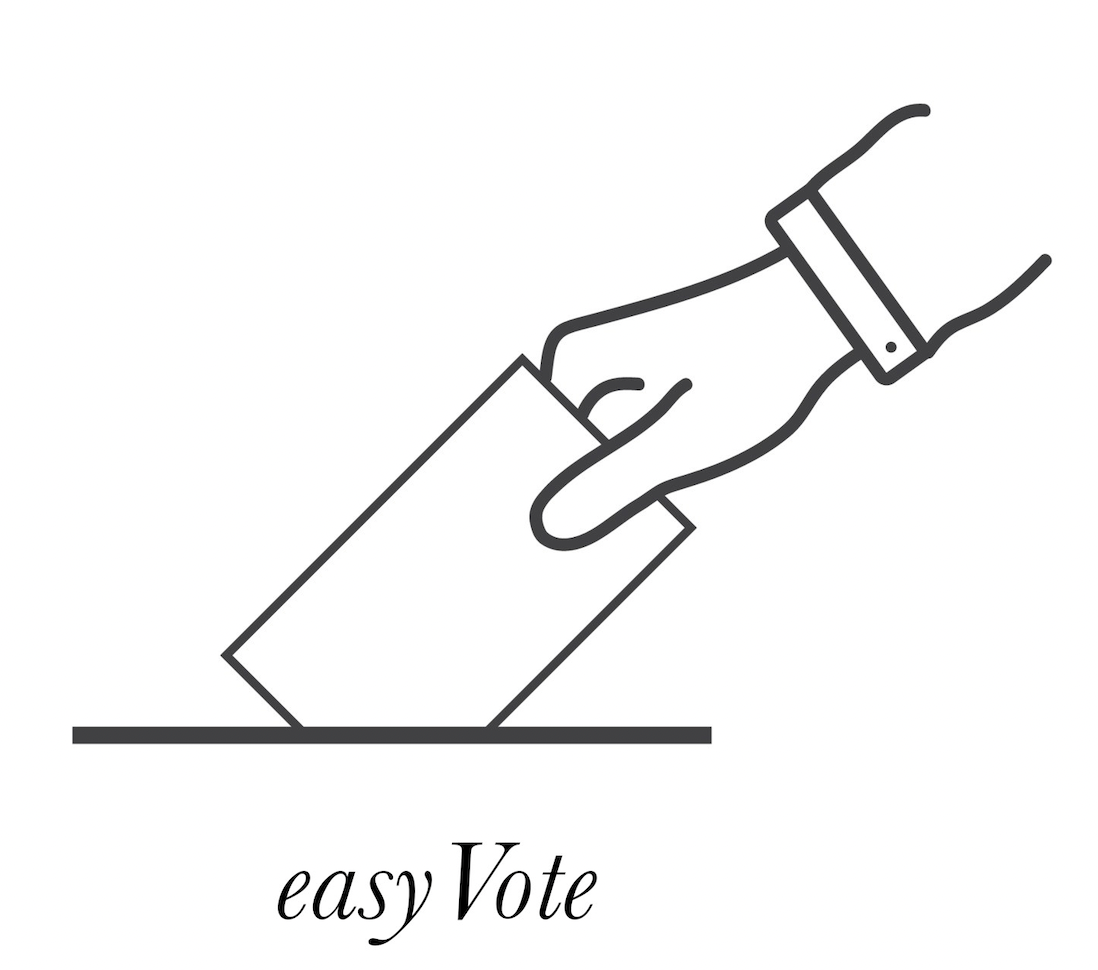
\includegraphics[scale=0.4]{images/logo.png}
\end{center}

\clearpage
\tableofcontents



\clearpage


\section{Introduction}

Democracy is a governmental model based of the belief that the population, or all eligible member of a state shall express their political intentions directly, or by electing representatives. 
easyVote is the new, efficient to use, comprehensive and dynamic electronic voting and balloting system. With easyVote governmental (and non) entities can expect to use an easy to comprehend system to manage electoral systems.
\subsection{Objectives:}
This RASD/SRS document shall include a glossary, general description, alongside a comprehensive specification of functional and non-function descriptions, use case diagrams, class diagrams, sequence diagrams, components diagrams, used design patterns section, database description, specification and validations with JML, user interface description section, testing section and installation and settings section.

\subsection{User Stories}
\begin{itemize}
\item As a voter in Milan, I want to be able to vote in the regional election at a distance so that I can ensure my and the other voters' safety.
\item As a governmental entity in Italy, I want to be able offer my citizens the possibility to vote exclusively  at a distance to mitigate the effects of the pandemic.
\item As a voter in the European Union, I want to be able to vote in the European election even while abroad.
\item As a voter in Argentina, I want to be able to vote in a national referendum without having to deal with an overly complicated UI.
\end{itemize}



\clearpage
\subsection{Terminology}
\begin{itemize}
\item easyVote: is a electronic voting system, for governmental and non governmental entities able to manage different voting systems
\item representatives: a person selected in an election to represent the political intention of the population
\item voter: a singular portion of the eligible voter population
\item electronic voting and balloting system: a voting and balloting system in which functions are primarily delegated to computers or computer infrastructure
\end{itemize}
\clearpage



\section{Requirements Specification}

easyVote is an electronic voting system, for governmental and non governmental entities able to manage different voting systems. Using easyVote eligible voters are able to vote in presence, or at a distance.
Different voting system include and are not limited to \begin{itemize}
\item ordinary vote: in which the voter is asked to order the candidates based on their preference
\item categorical vote: in which the voter is asked to select a preferred candidate among the candidates based on their preference
\item referendum: in which the voter is asked to express agreement or disagreement with the subject of the referendum 
\end{itemize}

\emph{When the voting process is complete, the result of the election is determined based on:}
\begin{itemize}
\item simple majority: the winning candidate is the one which received the majority of the votes
\item absolute majority: the winning candidate is the one which received 50\% + 1 votes
\item referendum without quorum: the votes are counted independently of the showing of the voter base
\item referendum with quorum: the votes are counted if and only if the majority of the eligible voter base voted
\end{itemize}
easyVote users shall be divided into voters and administrators. 
\subsection{Voters/users}
Voters must be able to vote in presence, or at a distance, using the easyVote portal, after a proper identification process, different based on the type of vote casted. \\If the vote is casted in presence, the identification process happens by requesting an identification document, if the vote is casted at a distance the identification process is delegated to the easyVote system.\\
Each voter is eligible to vote once, the vote is secret and cannot be reconnected to the caster.\\\\

\subsection{Administrators}

Administrator are special users able to configure new vote sessions. Vote session are characterised by  voting mode, voting session type, which include and are not limited to: ordinary voting session, categorical voting session, referendum voting session. \\

Administrator are also able to specify the candidates, set the start and the end of the election process, as well as displaying the winning candidate and/or the winning candidates.
\clearpage


\subsection{Functional Requirements}
\begin{itemize}
\item The easyVote system shall be clear, comprehensible and easy to use by every voter. Special measures shall be implemented to support voters with special conditions
\item Voter users shall register themselves through a dedicated easyVote portal 
\item Administrator users shall be authenticated using a dedicated easyVote portal
\item Administrator shall be able to create, manage, modify and display the results of an election
\item The easyVote system shall contain a manual to explain the different scrutinizing criteria
\item Ballots shall include images, text, icons, symbols to ease the recognition of the preferred candidate by a voter
\item The easyVote system shall recognise blank votes.
\item Ballots shall be recognised by the system if and only if the voter has specified a valid preference, or has expressed no preference at all (blank vote)
\item After the vote is casted a confirmation window shall be displayed to allow the voter to verify the correctness of the vote
\item A voter shall be able to verify his vote after the vote is casted
\item Users shall be able to resume a previously started voting sessions if the voting window has not closed yet
\item The easyVote system shall register all entities with a UID.
\item Administrators shall be able to create sample ballots for informative purposes.
\item The easyVote system shall provide appropriate information on the ballot for each candidate
\end{itemize}

\pagebreak


\subsection{Non-Functional Requirements}
\begin{itemize}
\item The code shall be commented according to "JAVADOC" guidelines;
\item The easyVote online portal shall only use the HTTPS protocol and never the HTTP protocol;
\item The drive on which the the easyVote system is installed shall have a level 6 RAID level for extra redundancy;
\item The easyVote portal shall be accessible through a web application light enough to be run on any digital device equipped with an Internet connection;
\item The easyVote system shall be impartial in all stages of use, the system shall never in any way influence the voter directly or indirectly;
\item The easyVote system shall guarantee a high degree of clearness and ease of use through the use of icons, symbols, images;
\item The easyVote system shall manage users and administrators information according to the GDPR guidelines.
\end{itemize}

\subsection{Security Requirements}
\begin{itemize}
\item If a voter is able to vote through multiple modes, the system shall recognise only the last vote casted;
\item A voter, to vote at a distance, shall identify himself with a high security protocol. The identification process shall be delegated to outside entities such as SPID;
\item The easyVote system shall never expose information regarding the voter, a vote casted, the administrators. This principle shall be respect during all stages use.
\end{itemize}

\pagebreak 


\section{Use case diagrams}

\begin{center}
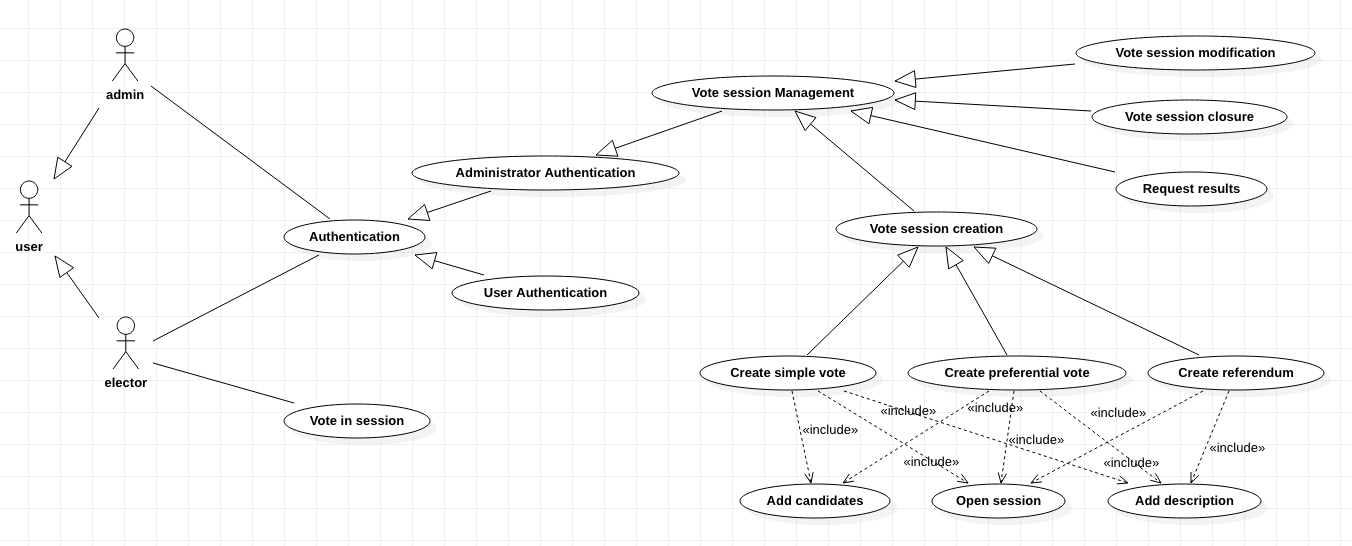
\includegraphics[scale=0.7]{images/usecaseDiagram.png}
\end{center}

\begin{itemize}
    \item Authentication: \\a use case accessed by admins and electors alike to authenticate themselves using their personal username and password selected during the registration process. \\
    The system keeps track of the authenticated user during the use of the program;
    \item Vote in session: \\a use case accessed by elector to vote in open session. The system automatically tracks and removes sessions in which the user has already voted in. The user can only accessed open voting sessions;
    \item Vote session management: \\a use case accessed by admins to manage voting session. By "manage voting session" we mean: vote session modification, vote session closure, vote session results request, vote session creation;
    \item Vote session modifications: \\a use case accessed by admins to add modifications to open vote sessions. Modification include and are not limited to: adding and removing candidates, changing a vote description;
    \item Vote session closure: \\a use case accessed by admins to close an open voting session;
    \item Request results:\\ a use case accessed by admins to request the result of a closed voting session;
    \item Vote session creation: \\a use case accessed by admins to request the opening of a new voting session. During the creation process the admin can define the following parameters and more: description, candidates, type of voting session;
    \item Create categorical vote: \\a use case accessed by admins to create a simple voting session. A simple voting session is a voting session in which the winning strategy is simple majority;
    \item Create ordinary vote: \\a use case accessed by admins to create a ordinary voting session. An ordinary voting session is a voting session in which a user is asked to select its favourite candidates in a descending order;
    \item Create referendum: \\a use case accessed by admins to create a referendum session. A referendum voting session is a voting session in which a user is asked to "in favour" or "not in favour" or leave blank ballot to a requested referendum change.
\end{itemize}

\clearpage

\subsection{Scenery descriptions}
In this section we look into the scenery description for the following actions:
\begin{itemize}
    \item Login
    \item Registration
    \item castVote
    \item Create voting session
    \item Modify voting session
    \item Vote in a referendum
    \item Request results
\end{itemize}

\begin{center}
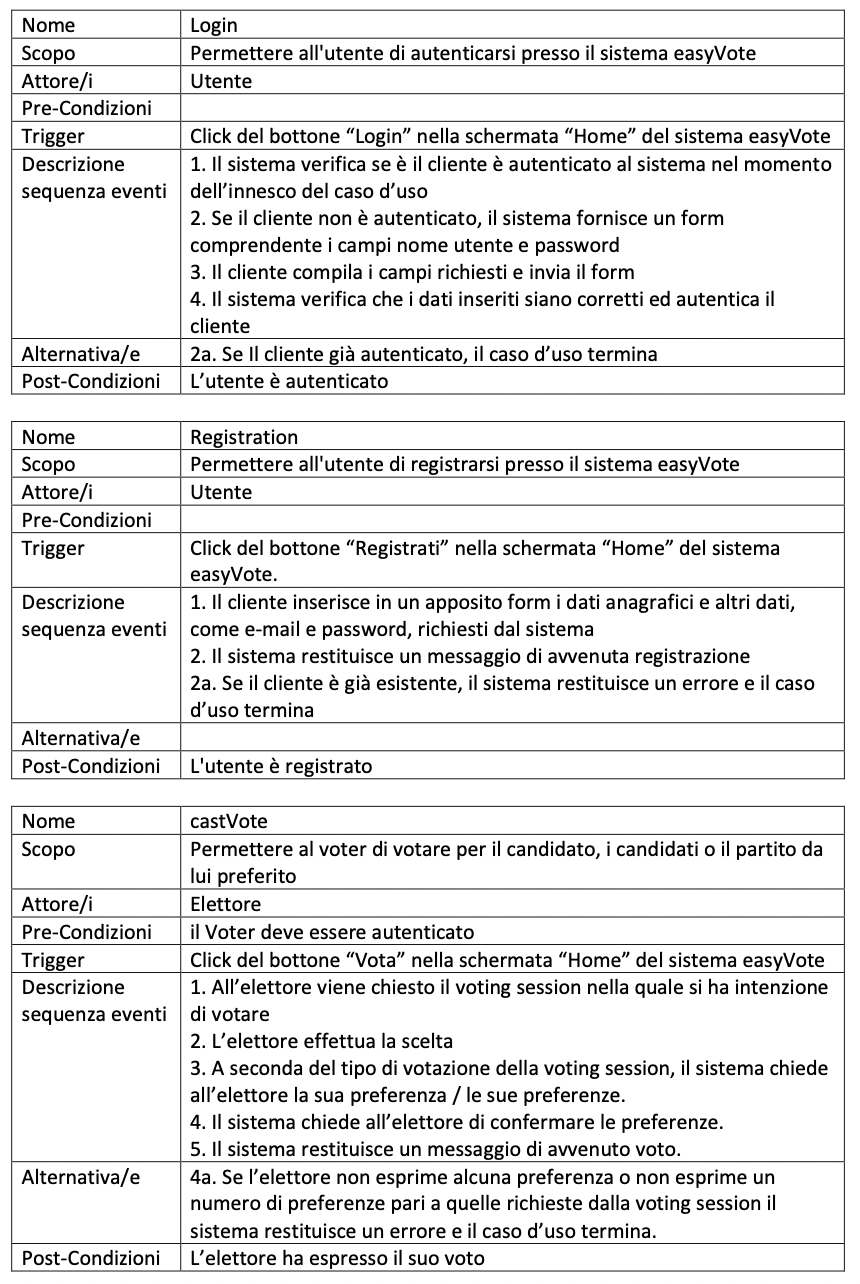
\includegraphics[scale=0.9]{images/sceneryDescription.png}
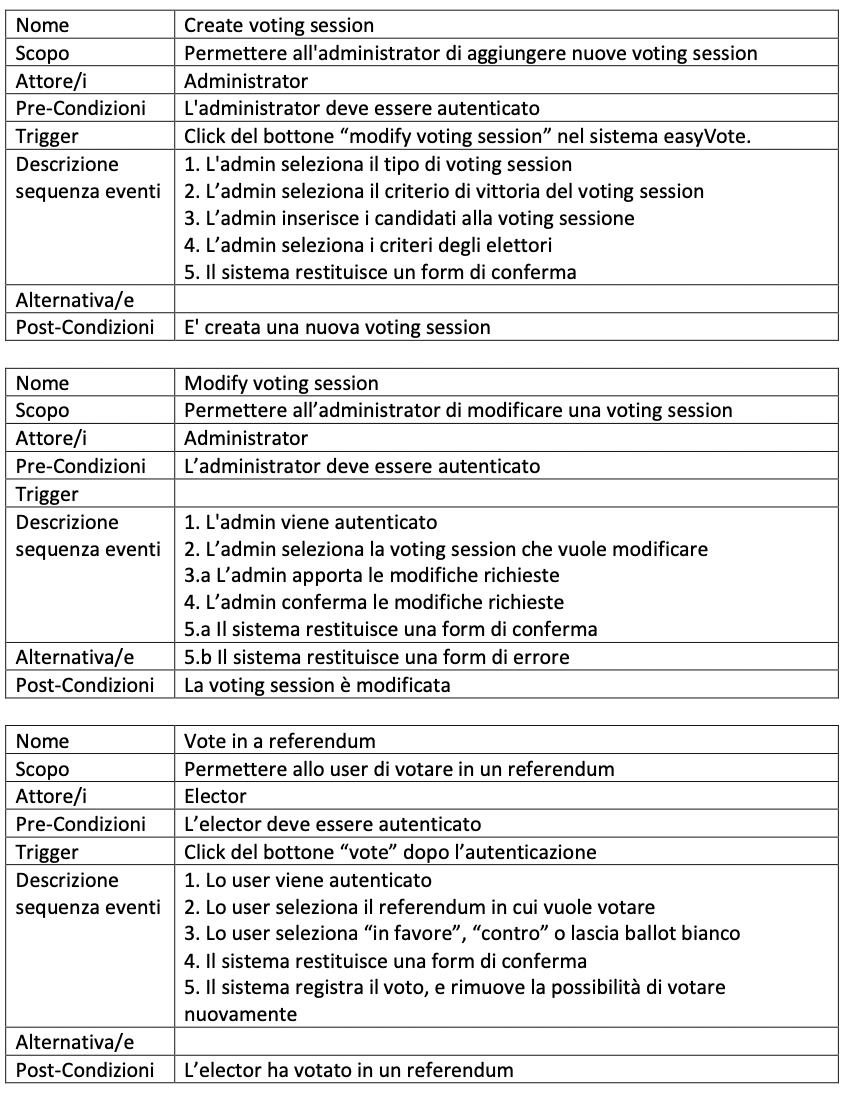
\includegraphics[scale=1]{images/sceneryDescription2.png}
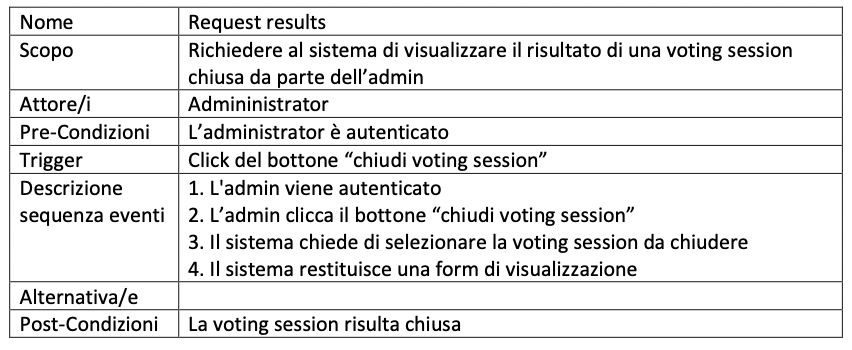
\includegraphics[scale=1]{images/sceneryDescription3.png}
\end{center}

\pagebreak

\section{Class diagrams}

\subsubsection{Controllers}
\begin{center}
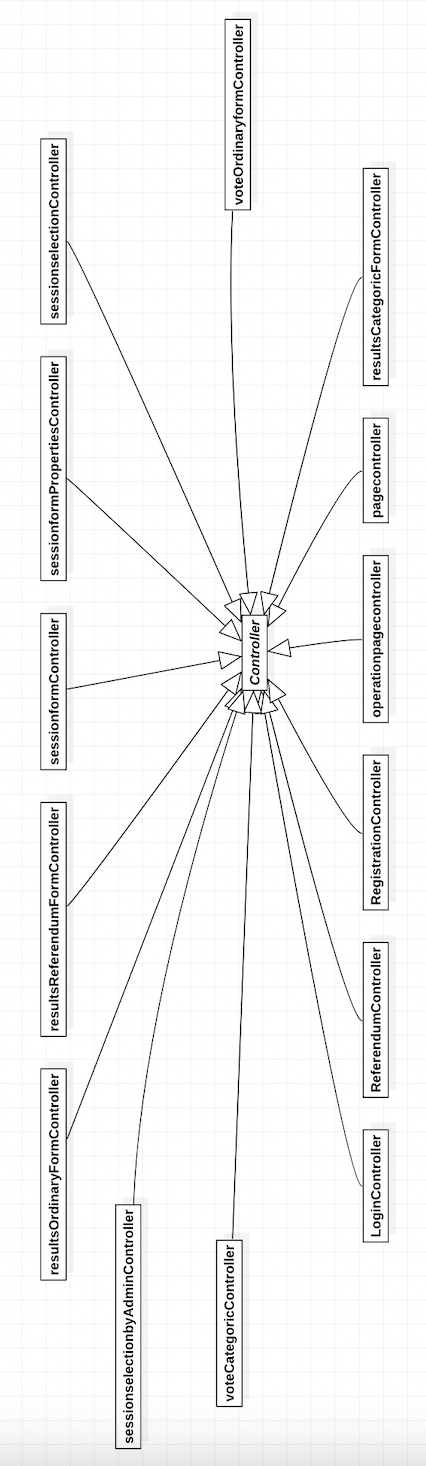
\includegraphics[scale=0.7]{images/class1.png}
\end{center}
\pagebreak

    \begin{center}
    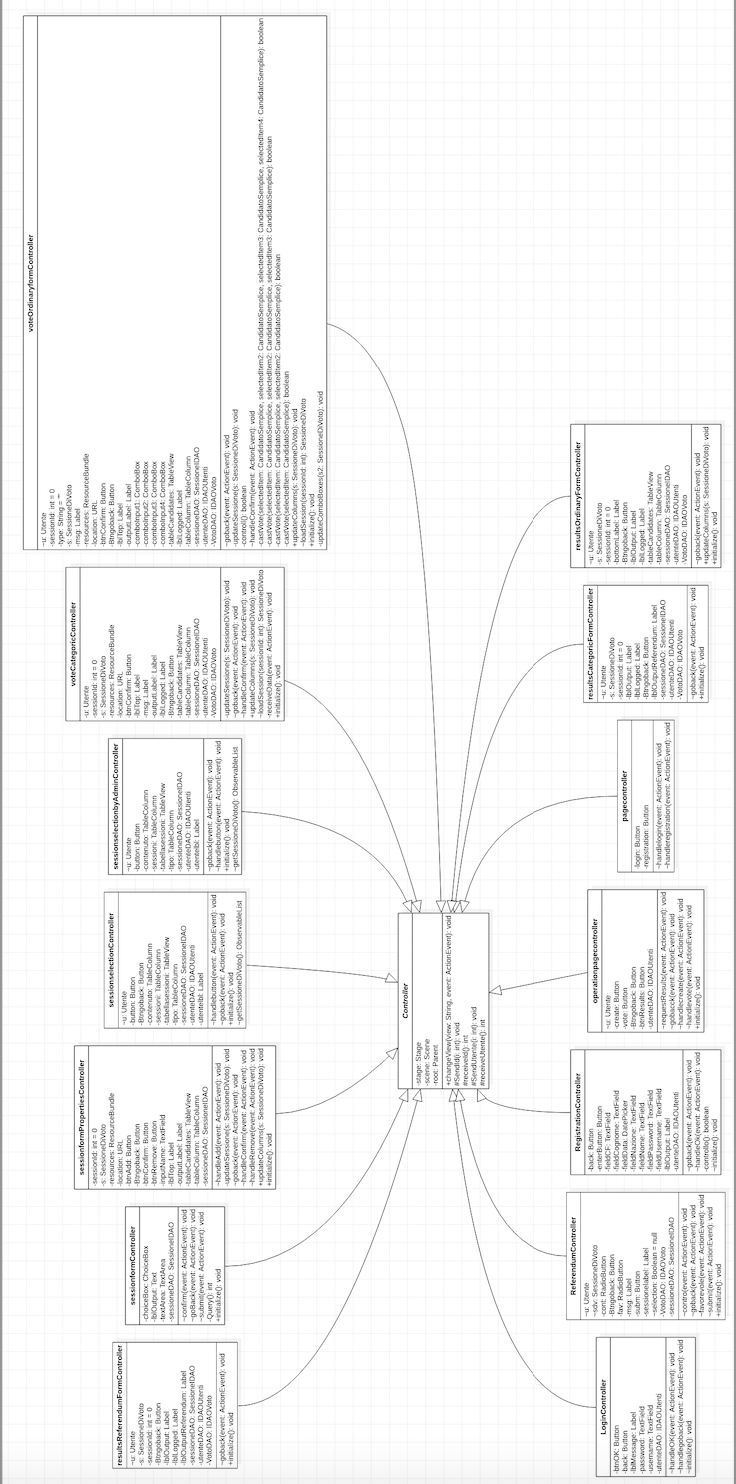
\includegraphics[scale=0.7]{images/class2.png}
    \end{center}

\pagebreak

\subsubsection{DAOs}
\begin{center}
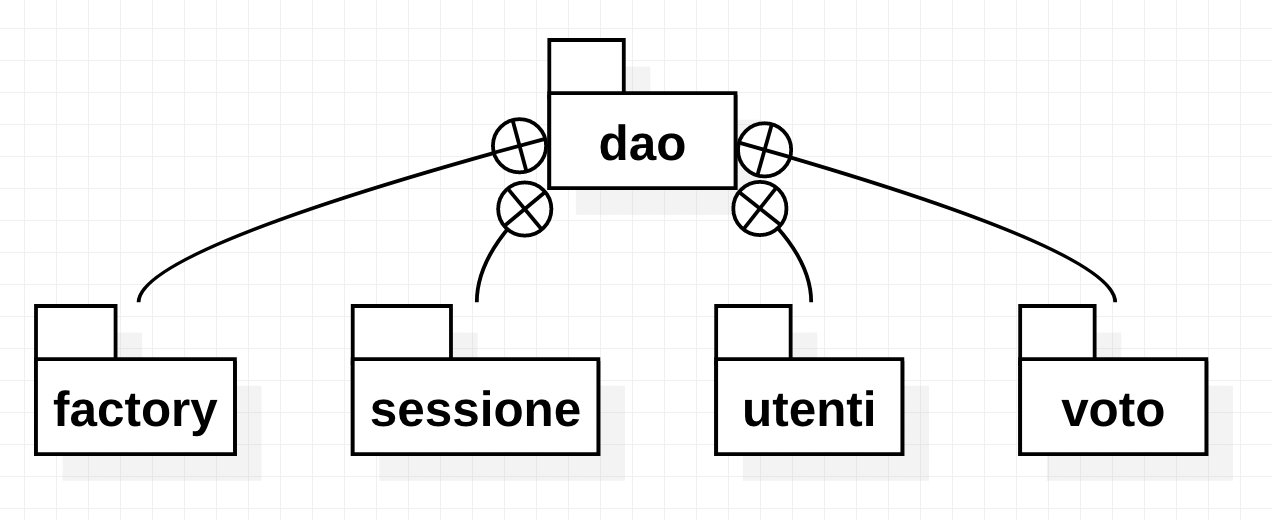
\includegraphics[scale=0.7]{images/class4.png}
\end{center}

\subsubsection{DAOs relationship}
\begin{center}
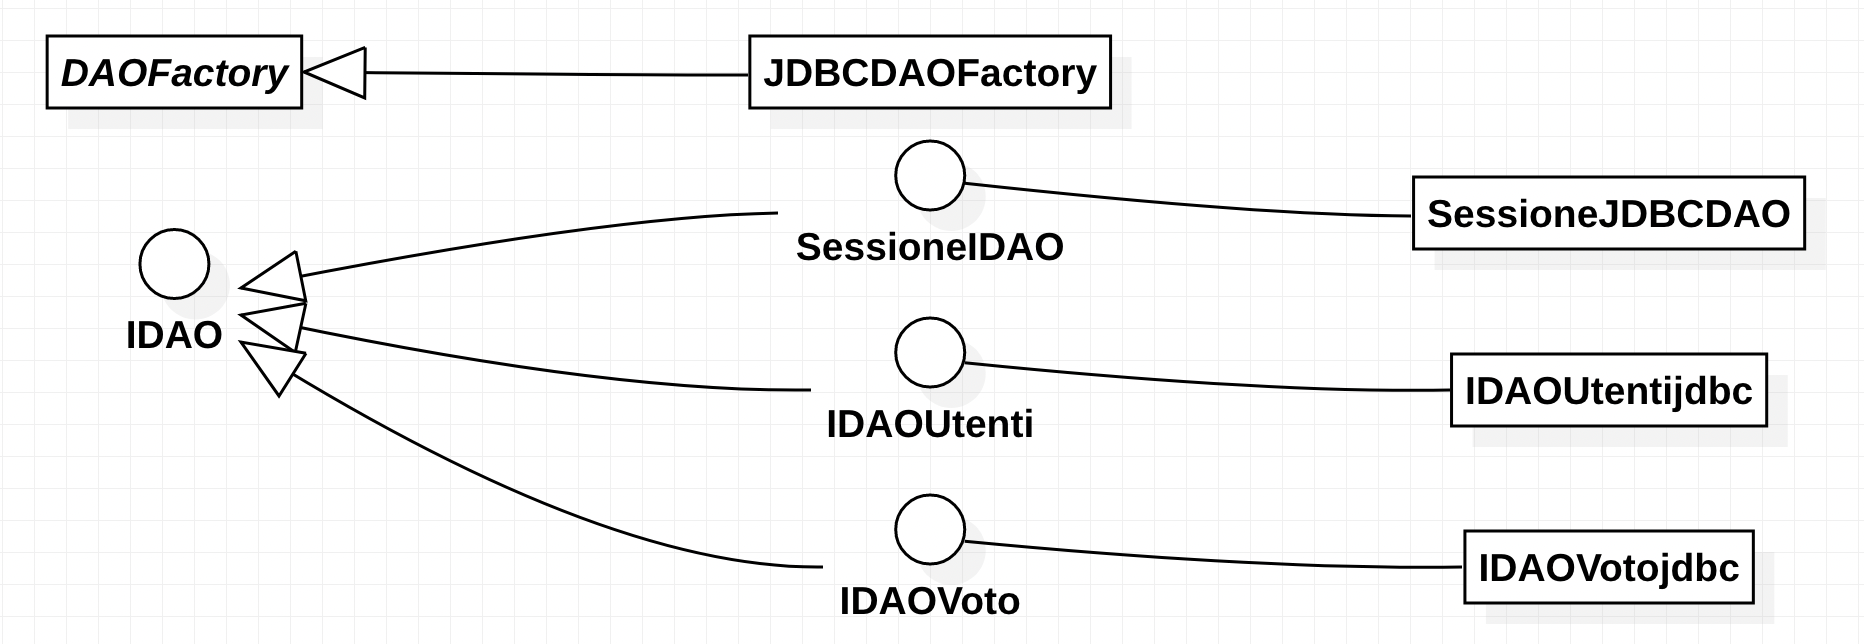
\includegraphics[scale=0.5]{images/class3.png}
\end{center}

\subsubsection{DAO Factory}
\begin{center}
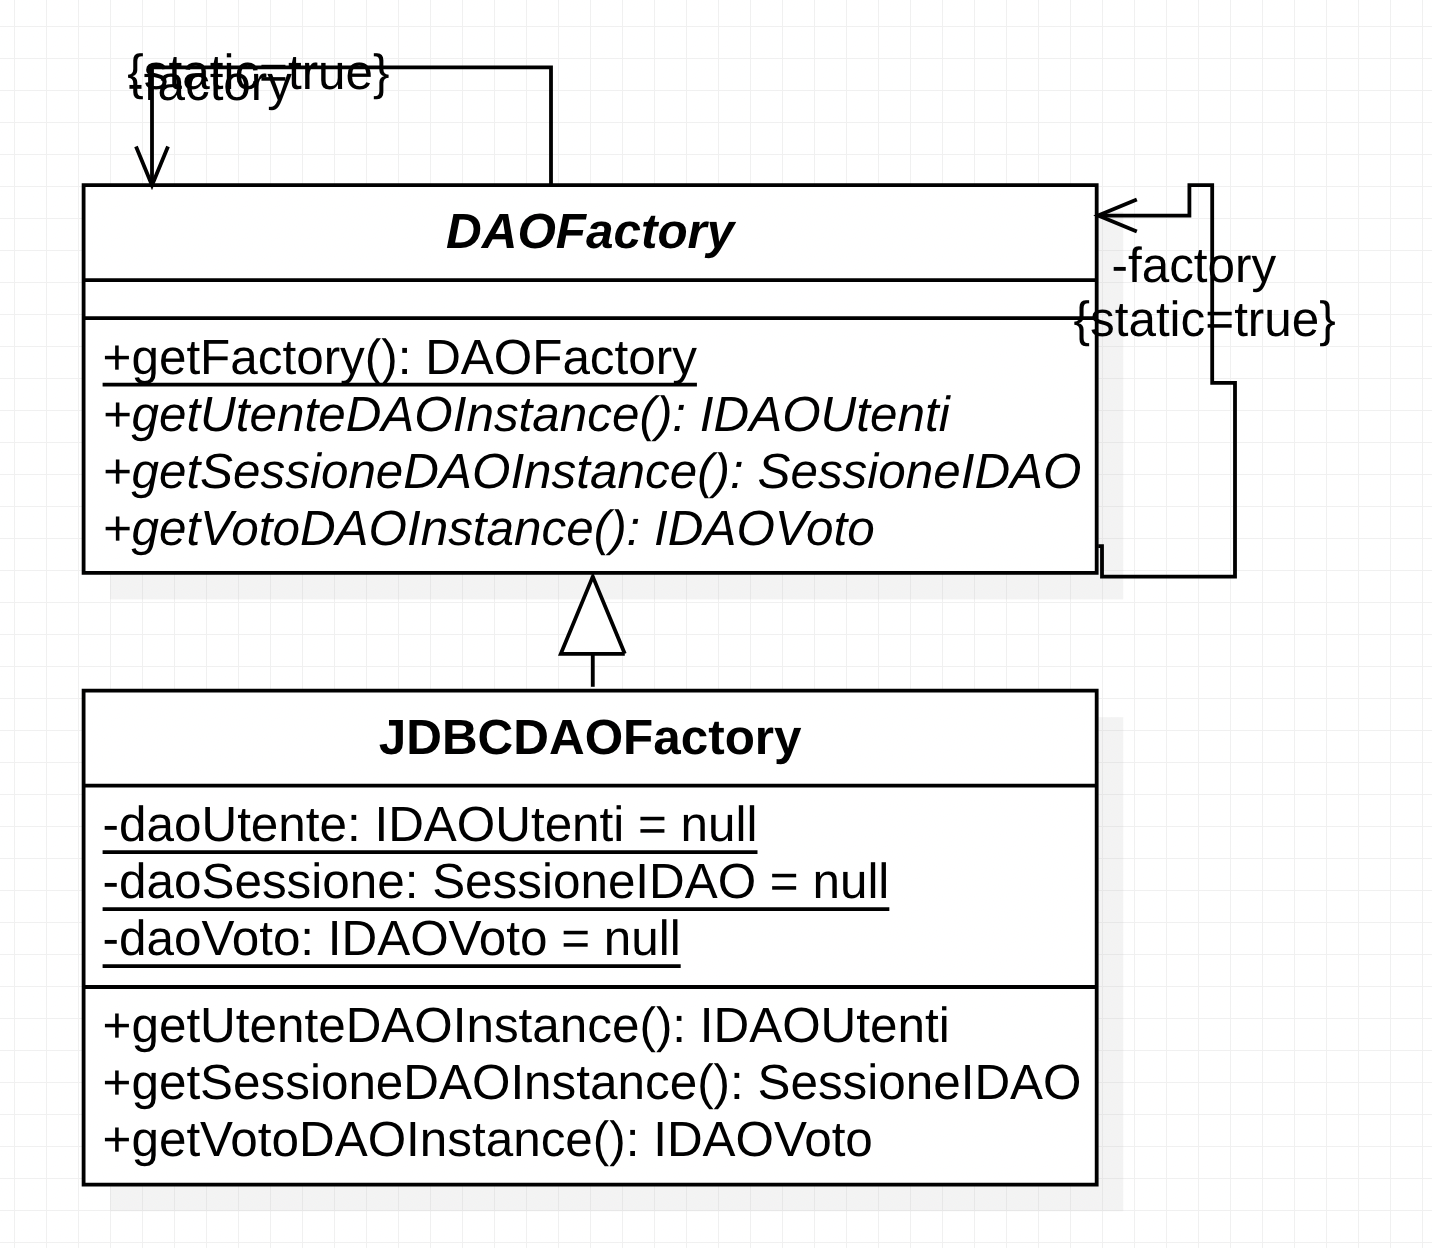
\includegraphics[scale=0.7]{images/class5.png}
\end{center}

\subsubsection{Sessione JDBCDAO}
\begin{center}
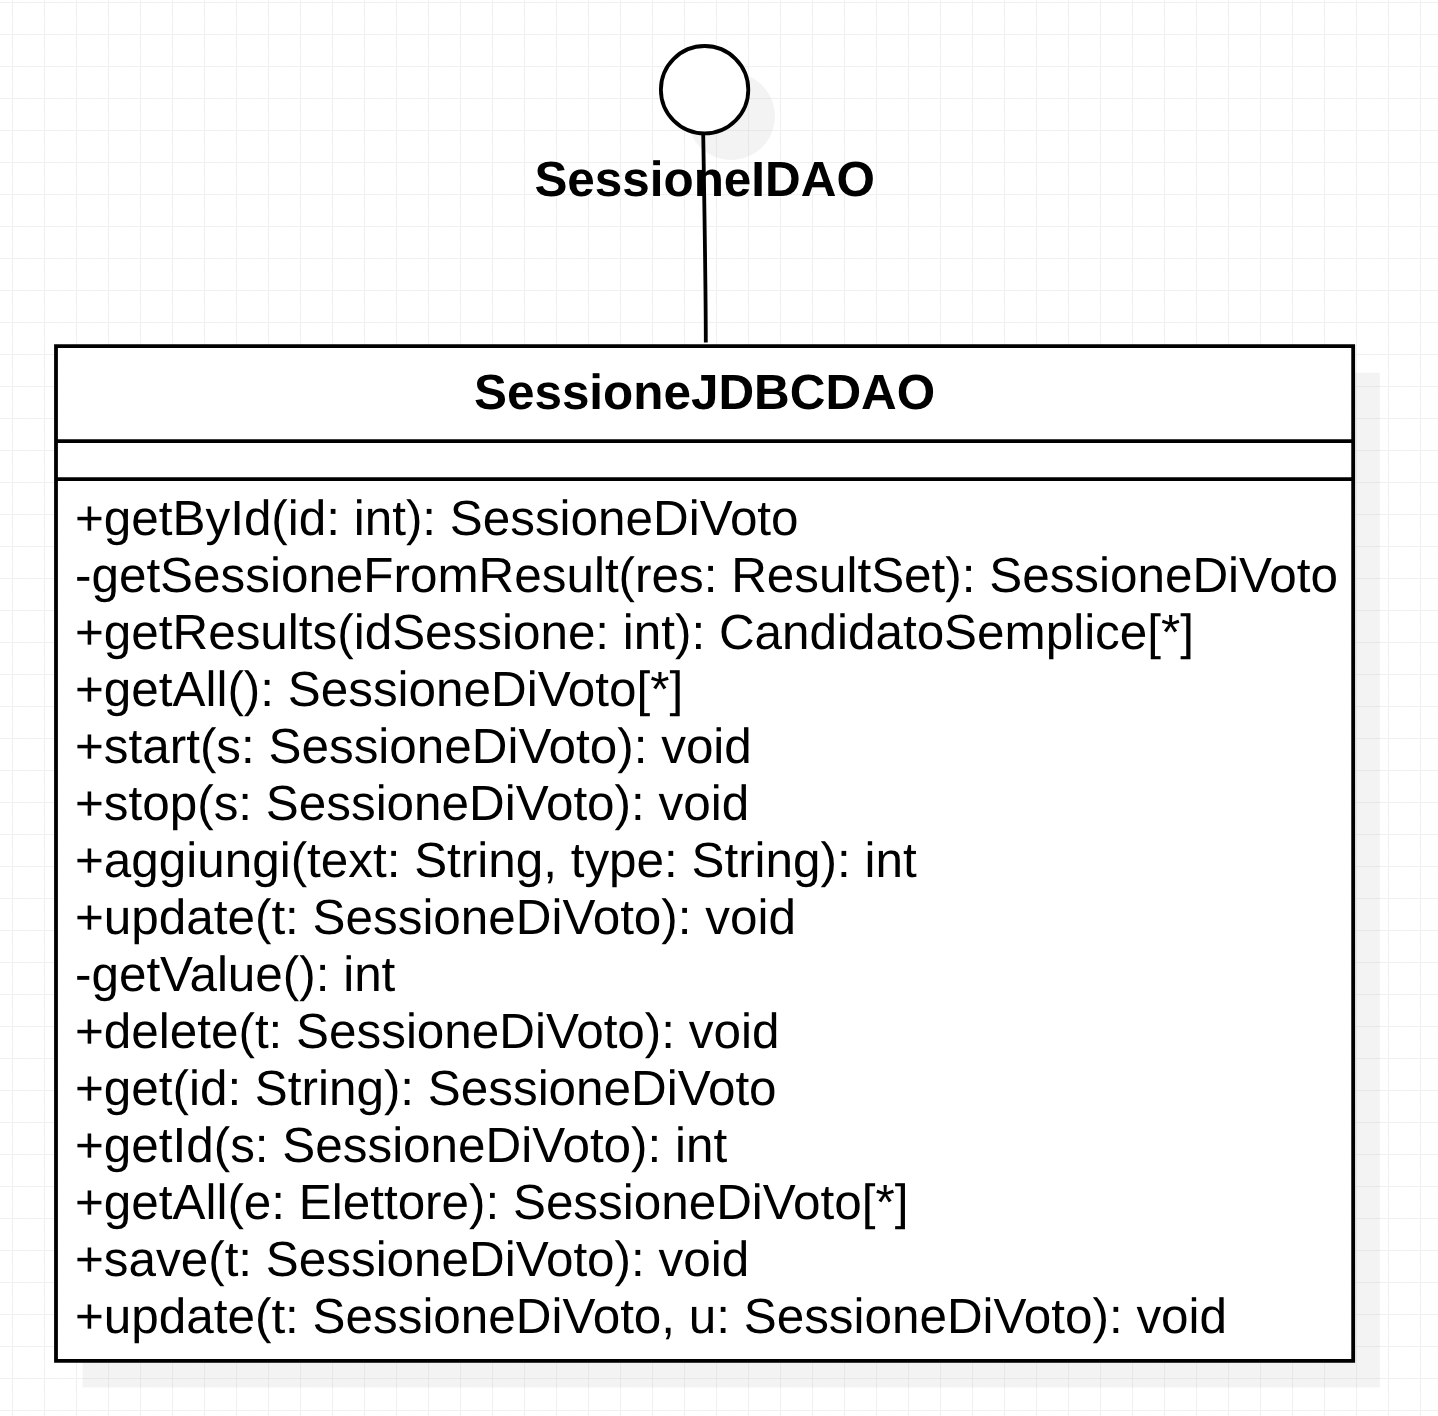
\includegraphics[scale=0.7]{images/class6.png}
\end{center}

\subsubsection{IDAOUtenti}
\begin{center}
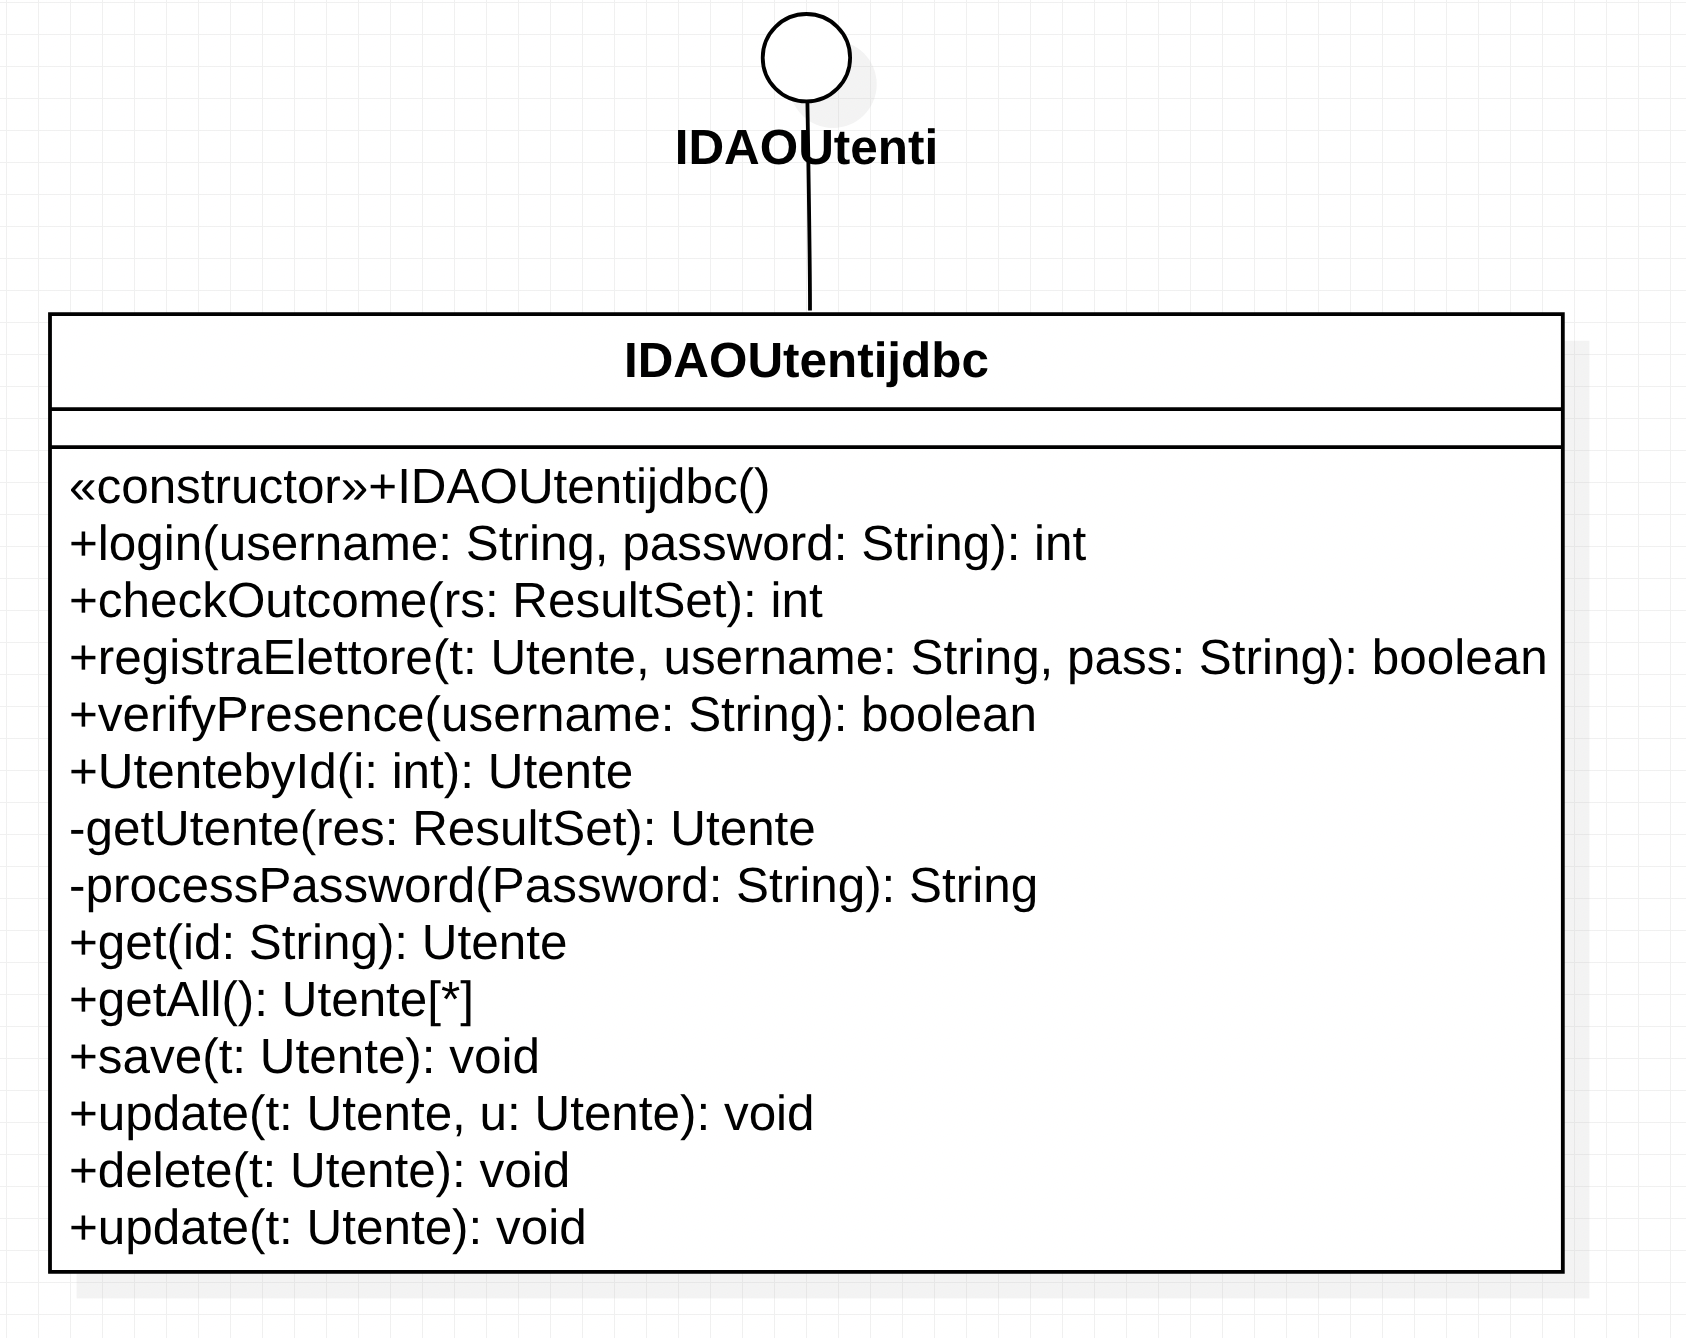
\includegraphics[scale=0.6]{images/class7.png}
\end{center}

\subsubsection{IDAOVoto}
\begin{center}
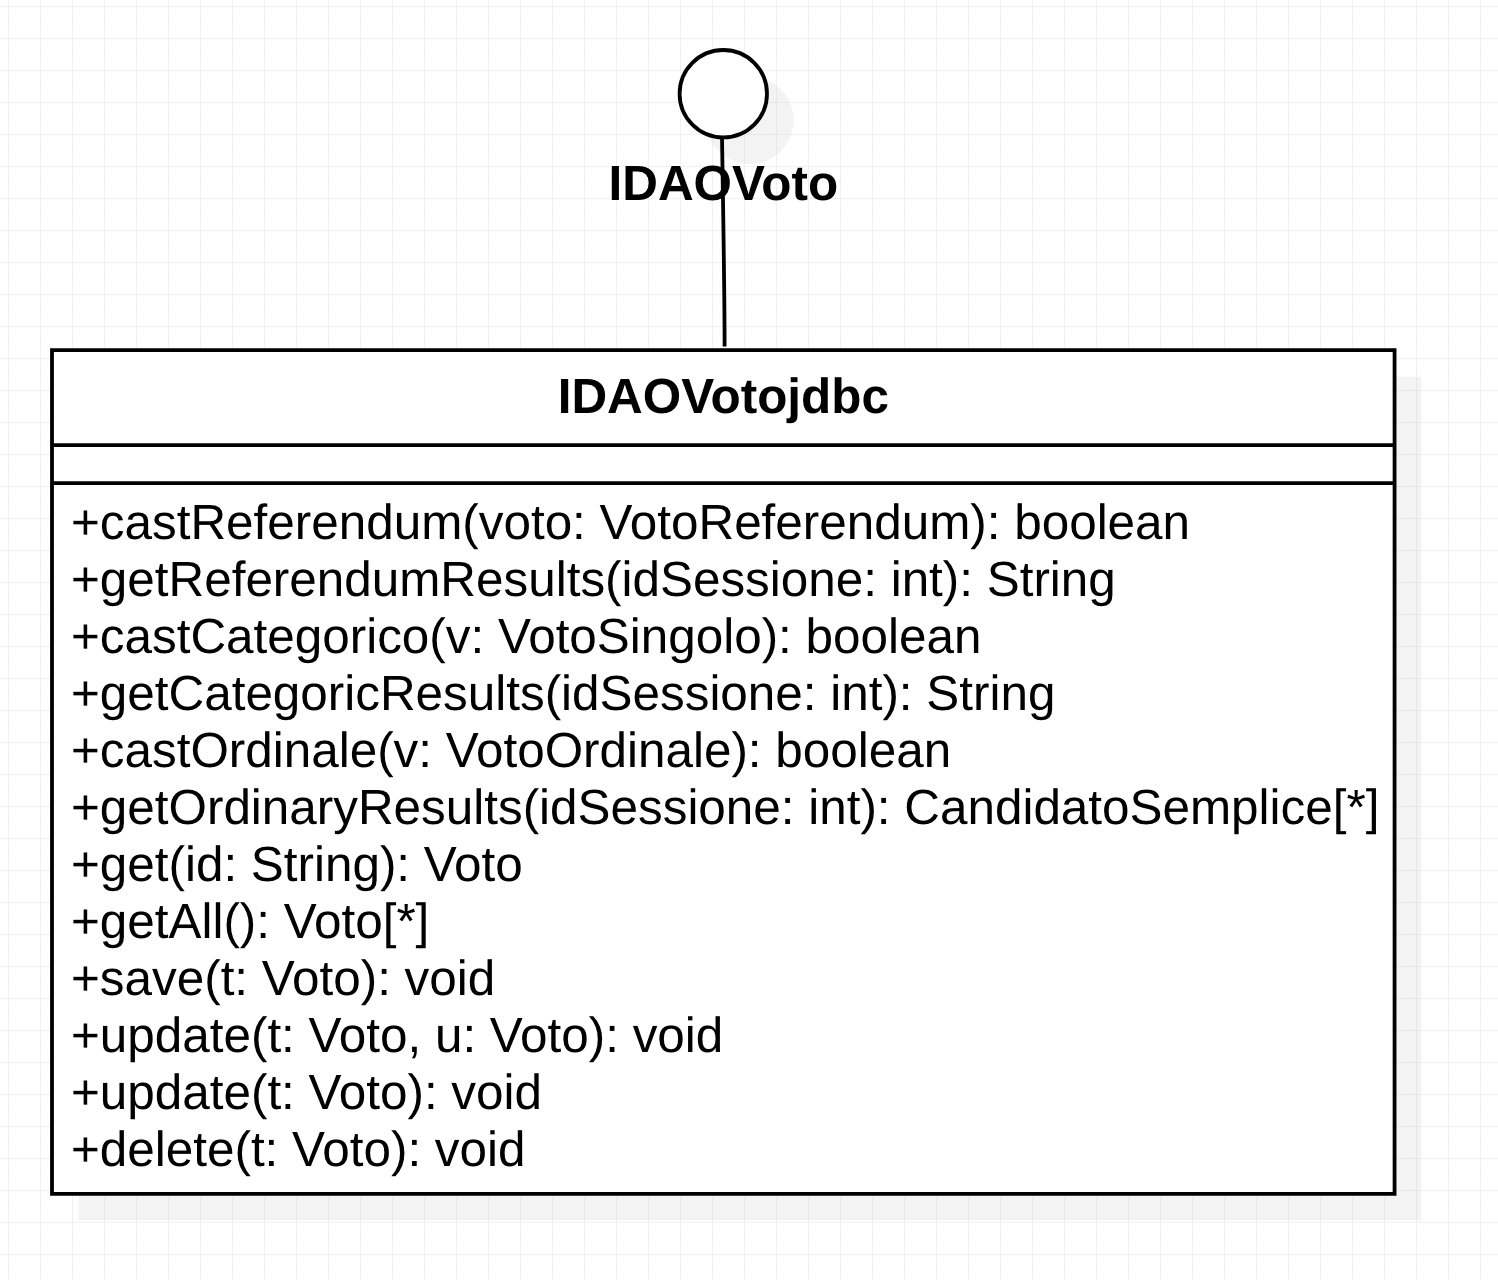
\includegraphics[scale=0.7]{images/class8.png}
\end{center}

\pagebreak

\subsubsection{Database Manager}
\begin{center}
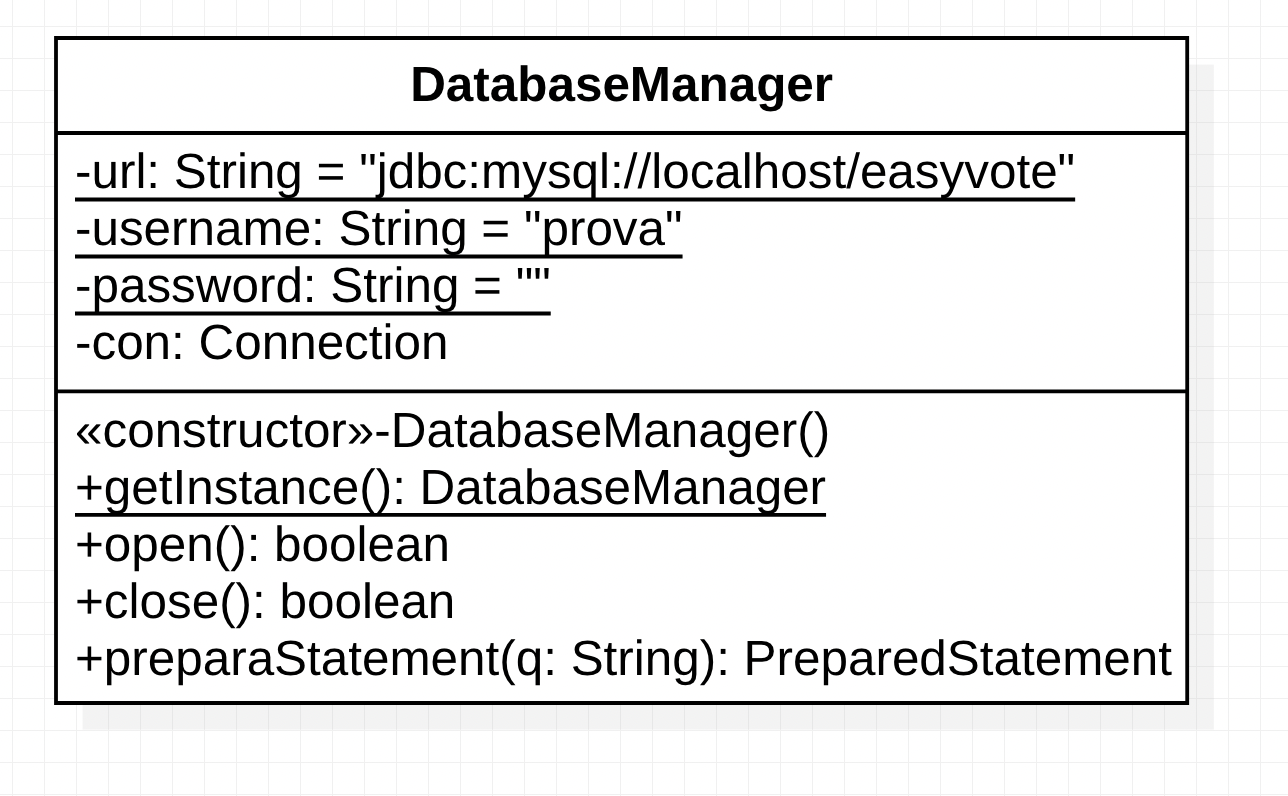
\includegraphics[scale=0.7]{images/class9.png}
\end{center}
\pagebreak


\subsubsection{Utenti \& Voto}
\begin{center}
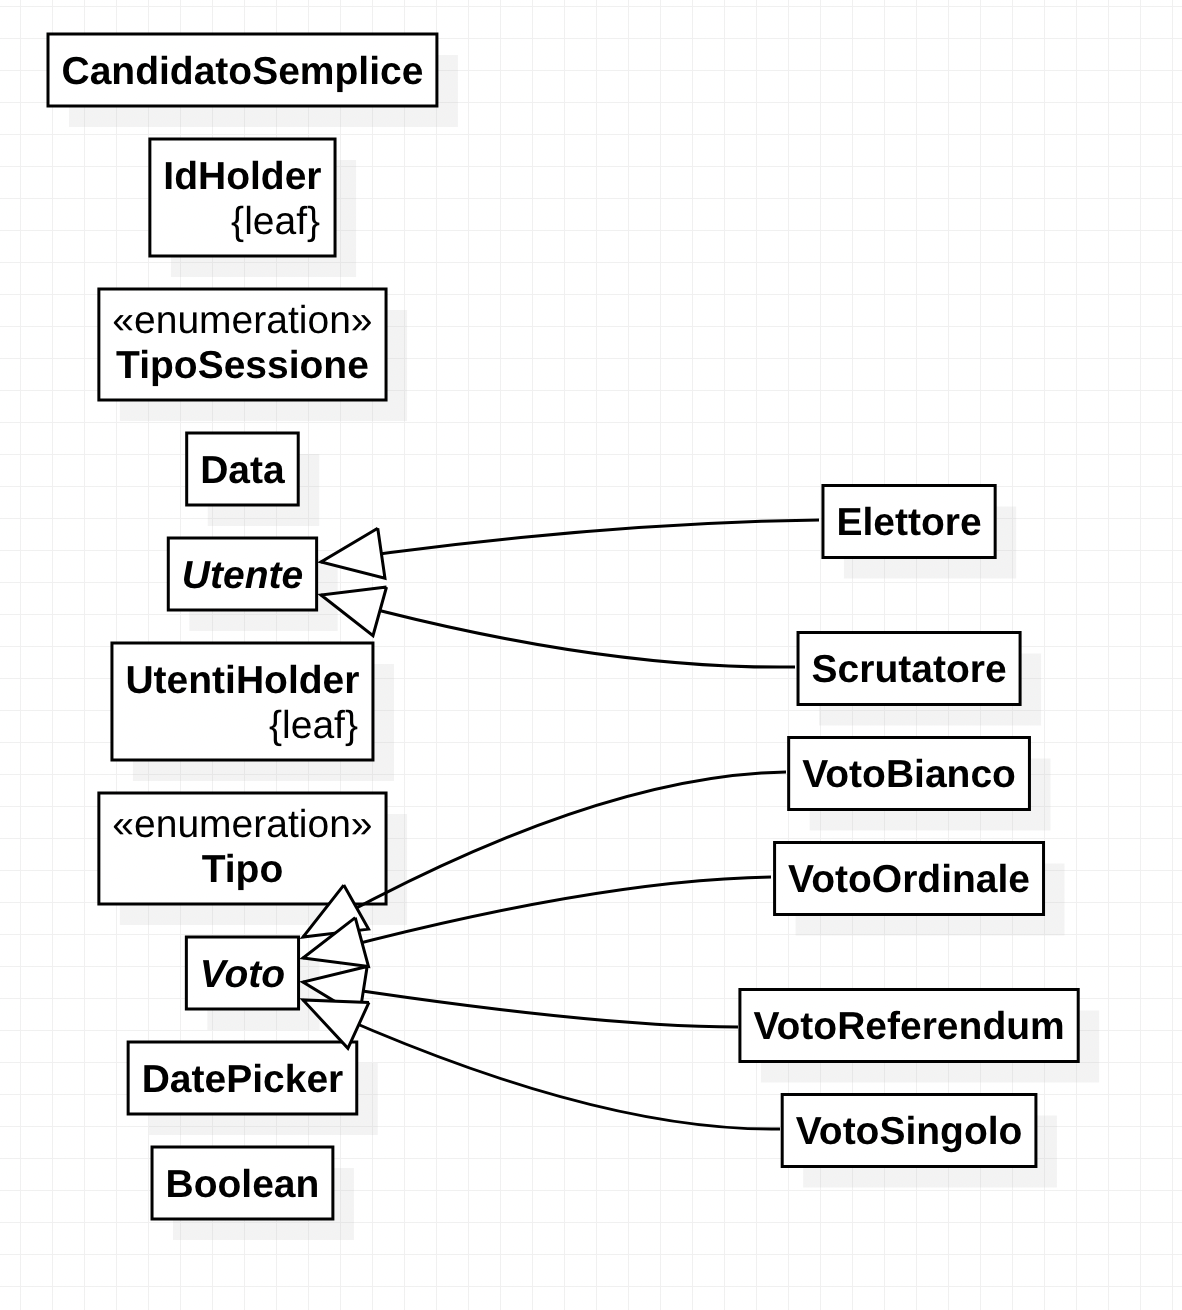
\includegraphics[scale=0.7]{images/class10.png}
\end{center}


\subsubsection{Utente}
\begin{center}
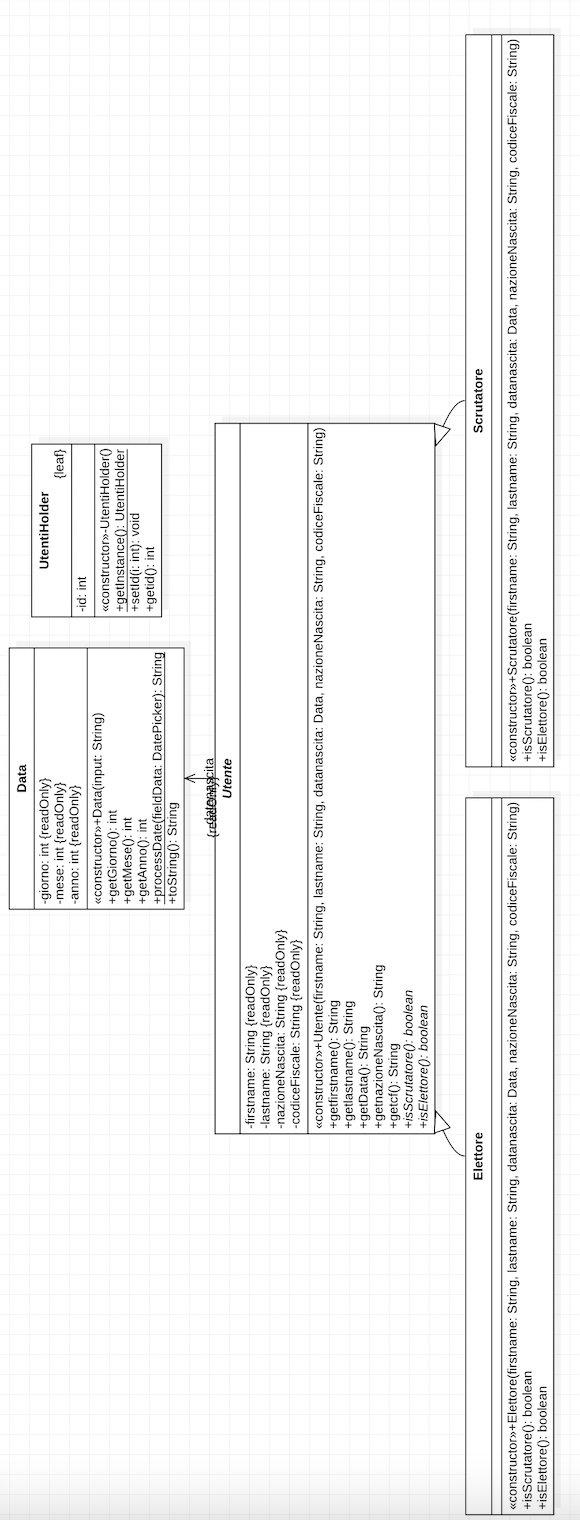
\includegraphics[scale=0.7]{images/class12.png}
\end{center}
\subsubsection{Session Holder}
\begin{center}
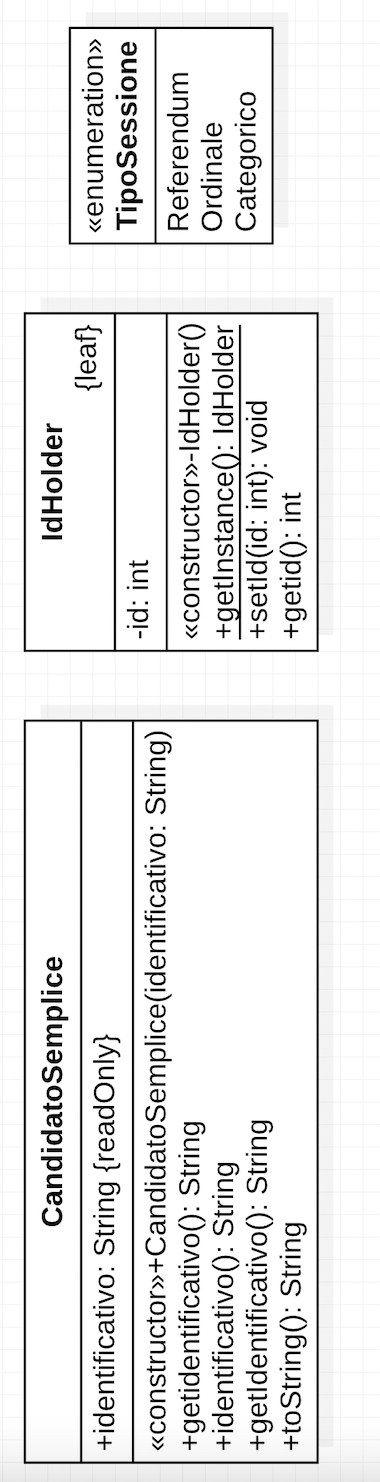
\includegraphics[scale=0.6]{images/class11.png}
\end{center}
\subsubsection{Voto}
\begin{center}
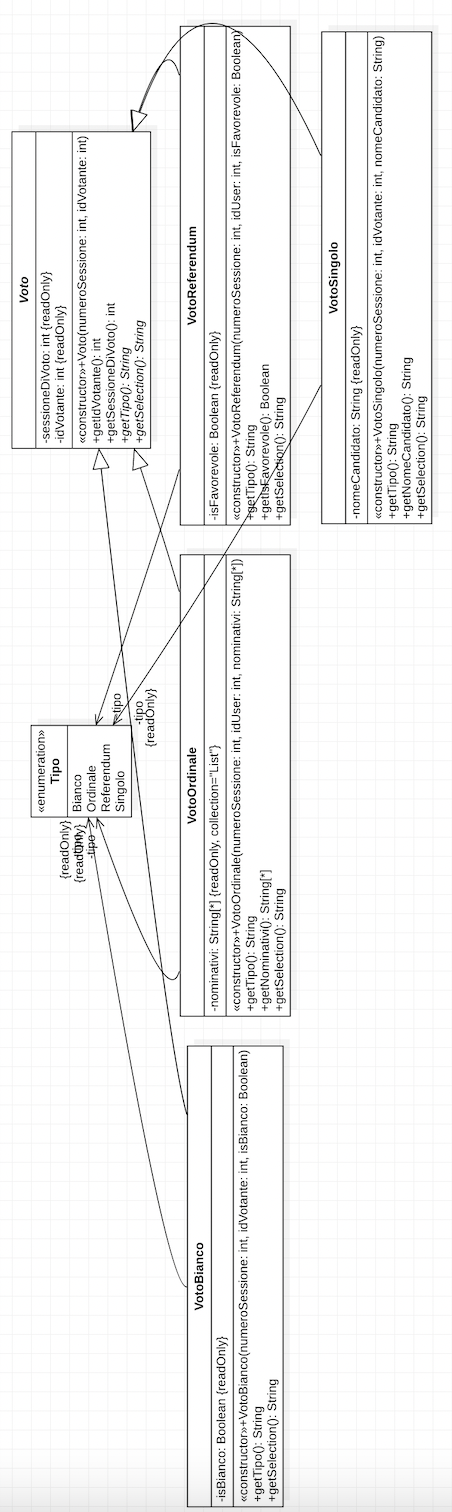
\includegraphics[scale=0.7]{images/class13.png}
\end{center}


\section{Sequence diagrams}
\subsection{Login}
    \begin{center}
    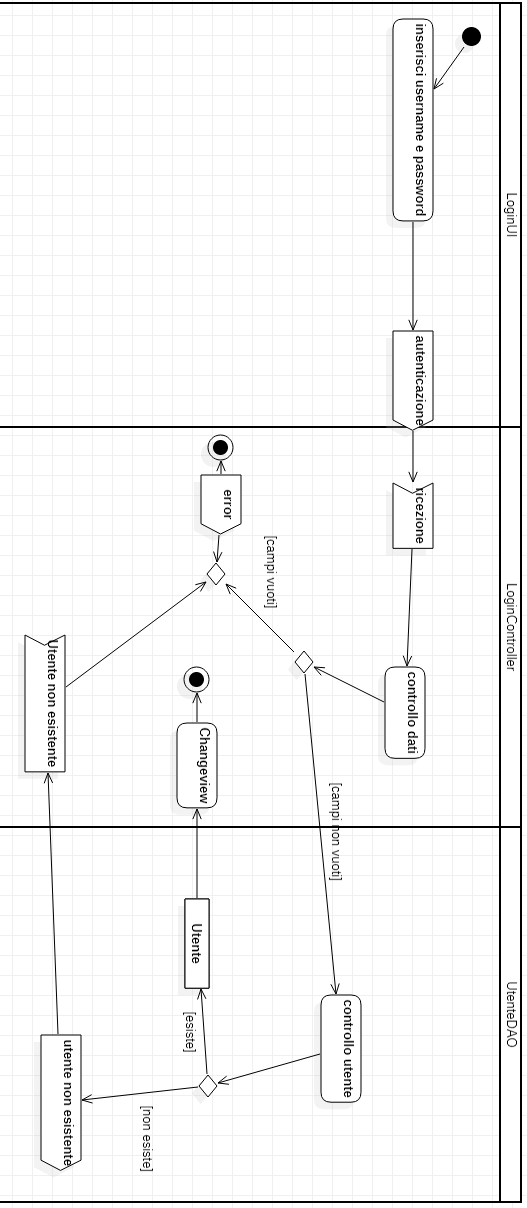
\includegraphics[scale=0.5]{images/loginactivity.png}
    \end{center}
    \pagebreak

\subsection{Vote}
\subsubsection{Referendum}
    \begin{center}
    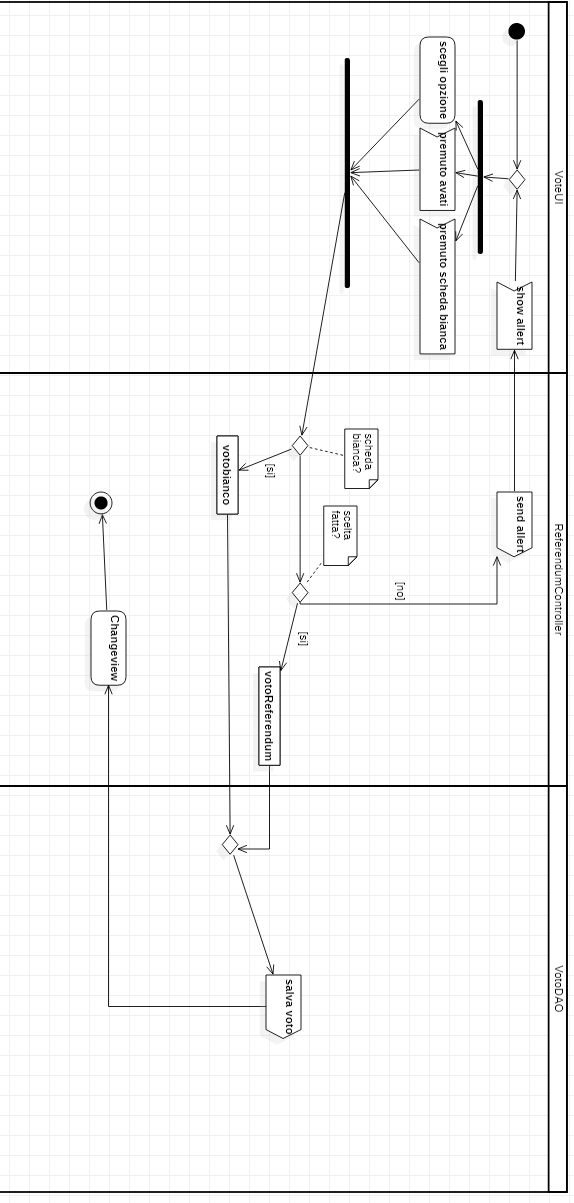
\includegraphics[scale=0.5]{images/ReferendumActivity.png}
    \end{center}
    \pagebreak
\subsubsection{Categorical}
    \begin{center}
    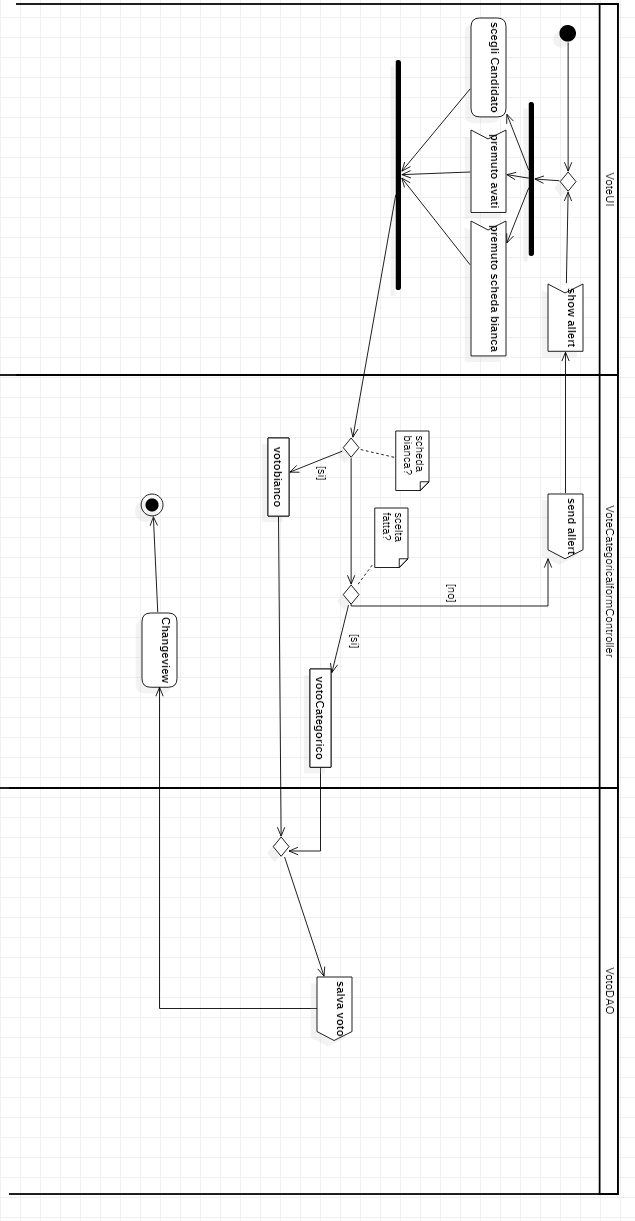
\includegraphics[scale=0.5]{images/Categoricalactivity.png}
    \end{center}
    \pagebreak
    
    
\section{Components diagrams}
\subsection{An overview of the components and their interactions}
\begin{center}
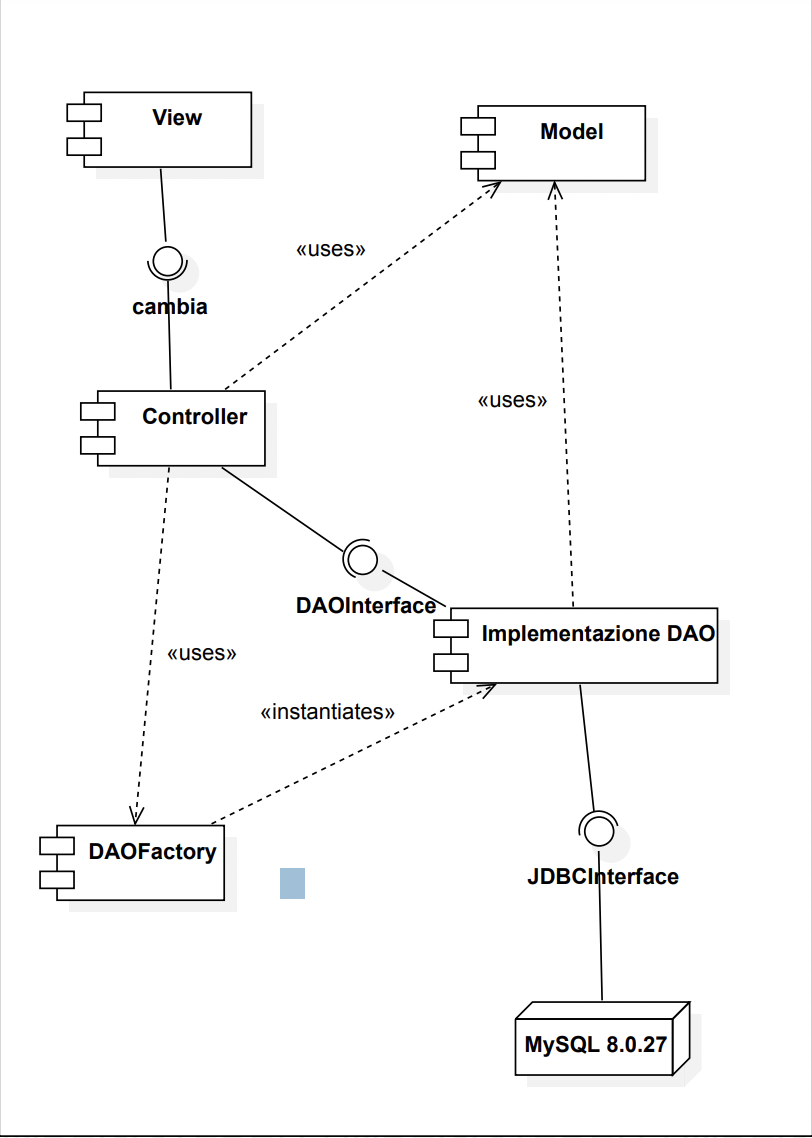
\includegraphics[scale=0.8]{images/componentDiagram.png}
\end{center}


\section{Design patterns employed}
\subsection{Singleton}
The "Singleton" pattern is a software design pattern which aims to restrict the istantiation of a class to a single instance. One object is instantiated and spread across classes to coordinate actions.\\
The singleton pattern is utilized to spread the \emph{SessioneDiVoto} with the \emph{SessioneIDAO} class and the \emph{Utente} with the \emph{IDAOUtenti} class.

\subsection{DAO}
The "DAO pattern" o "Data Access Object" is structural pattern to isolate the application layer from the database layer.\\

The "DAO pattern" is combined with the Abstract factory pattern to hide complexities related to accessing databases to specific classes, leaving there the definition of specific implementations. 
The "DAO pattern" are organized under \emph{easyVote.DAO}, and are \emph{easyVote.DAO}, \emph{easyVote.DAO.factory}, \emph{easyVote.DAO.sessione}, 
\emph{easyVote.DAO.utenti},  \emph{easyVote.DAO.voto},  \emph{easyVote.database}.

\subsection{MVC}
The "MVC model" o "Model-View-Controller" is a software design pattern used to develop user interfaces that divides program logic into three interconnected elements.\\

The easyVote software is divided in models, controllers and views. The file structure is organized under \emph{easyVote.models}, \emph{easyVote.controllers}, \emph{easyVote.views}, \emph{easyVote.DAO}, \emph{easyVote.database} and \emph{easyVote.factory}. This is done to separate internal representations and to present data in intuitive and easy to use way to both the programmer and the user.
\subsection{Abstract factory}
The "Abstract factory" is a design pattern which aims to encapsulate object creation in a separate object, this is done to facilitate the implementation of new features.
The easyVote software used this design pattern to facilitate the creation of new "DAO" classes.

\pagebreak

\section{Database description}
The easyVote database was designed from the ground up with simplicity and easy of use in mind. The DBMS chosen was the "MySQL" Database due to its widespread use, ease of connectivity, and the way the "JDBC" library allows for a seamless experience.

The tables present in the easyVote Database are: "voto", "session", "users".
\pagebreak

\subsection{users}
The "users" table's job is to encapsulate all the information regarding a easyVote user such as:
\begin{itemize}
    \item iduser: a user's automatically generated id number;
    \item name: a user's inserted name;
    \item lastname: a user's inserted surname;
    \item birthdate: a user's inserted birthdate;
    \item codicefiscale: a user's inserted and system checked "codice fiscale" or vat code number;
    \item username: a user's chosen username used to login;
    \item password: a user's chosen password hashed using the "SHA-256" secure hashing algorithm;
    \item isadmin: to identify if the user is an admin or not.
\end{itemize}
The primary key is "iduser" and there are no secondary keys.\\

The database state at the moment of testing was: 
    \begin{center}
    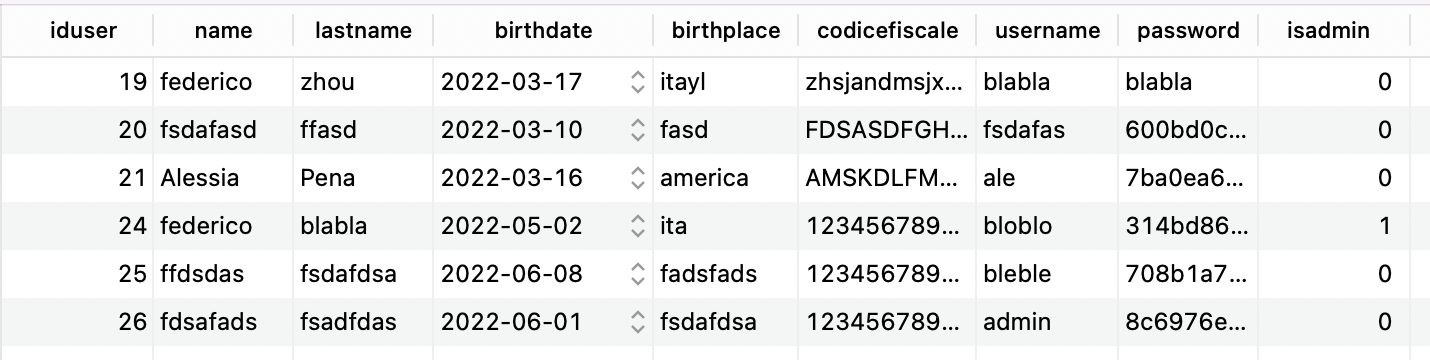
\includegraphics[scale=0.5]{images/voto2.png}\\
    \emph{The "users" table}
    \end{center}
    
    
\pagebreak

\subsection{session}
The "session" table's job is to encapsulate all the information regarding a vote session such as:
\begin{itemize}
    \item id: a session's automatically generated id number;
    \item text: an admin inserted session text description;
    \item candidato: an admin inserted and system factored JSON type text which identifies the candidates;
    \item isOpen: a session's attribute to define if the session is open or not;
    \item type: an admin inserted attribute to identify the session's type.
\end{itemize}
The primary key is "id" and there are no secondary keys.\\

The database state at the moment of testing was: 
    \begin{center}
    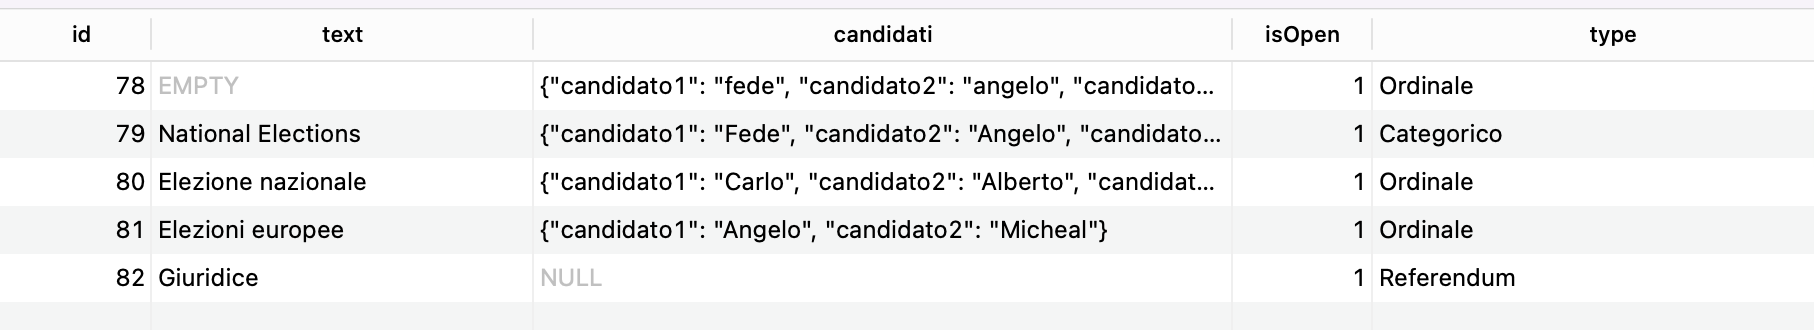
\includegraphics[scale=0.5]{images/voto1.png}\\
    \emph{The "session" table}
    \end{center}

\pagebreak

\subsection{voto}
The "voto" table's job is to encapsulate all the information regarding a session vote such as:
\begin{itemize}
    \item idSession: a system inserted valid id session number;
    \item idUser: a system inserted valid idUser number;
    \item selection: a system generated JSON type text which identifies an idUser's selection for a idSession vote session.
\end{itemize}
The primary keys are "idSession" and "isUser" and there are no secondary keys.\\

The database state at the moment of testing was: 
    \begin{center}
    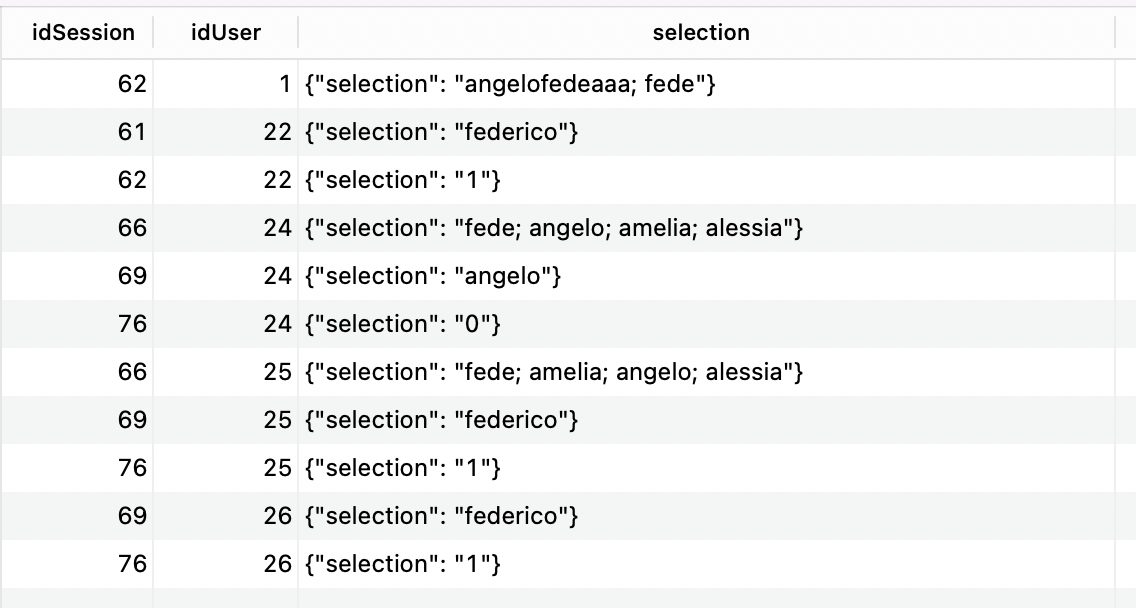
\includegraphics[scale=0.5]{images/voto3.png}\\
    \emph{The "voto" table}
    \end{center}

\pagebreak

\section{Deployment diagram}
\begin{center}
    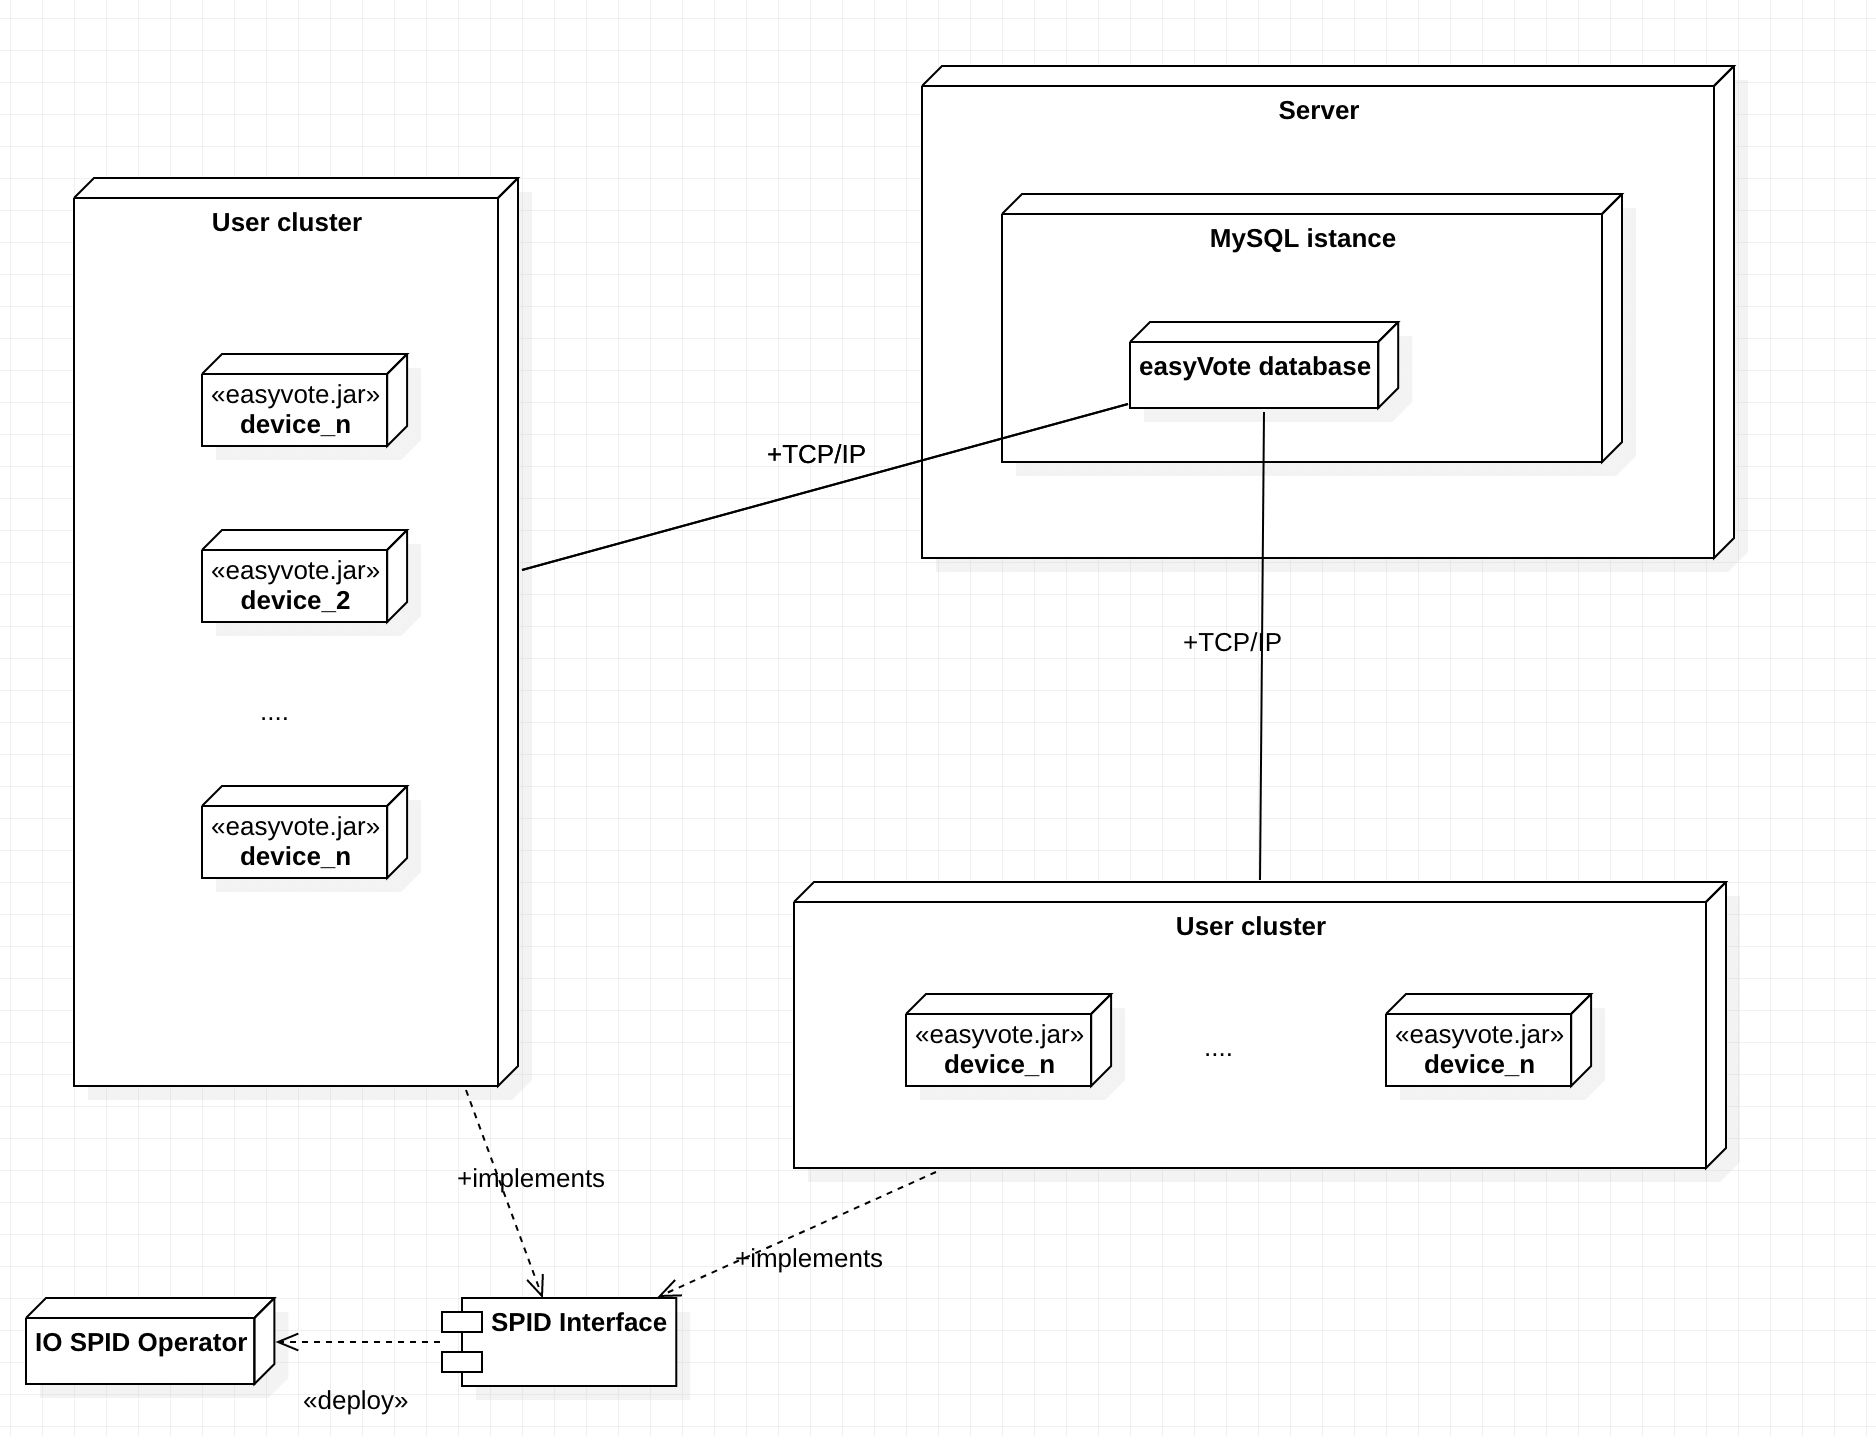
\includegraphics[scale=0.5]{images/deployment.png}\\
    \emph{easyVote's deployment diagram}
    \end{center}
The SPID interface's job is to facilitate communication between easyVote applications and the "IO SPID Operator" which provides high level security authentication to easyVote's terminal.
    \pagebreak
    
\section{UI description diagram}
\begin{center}
    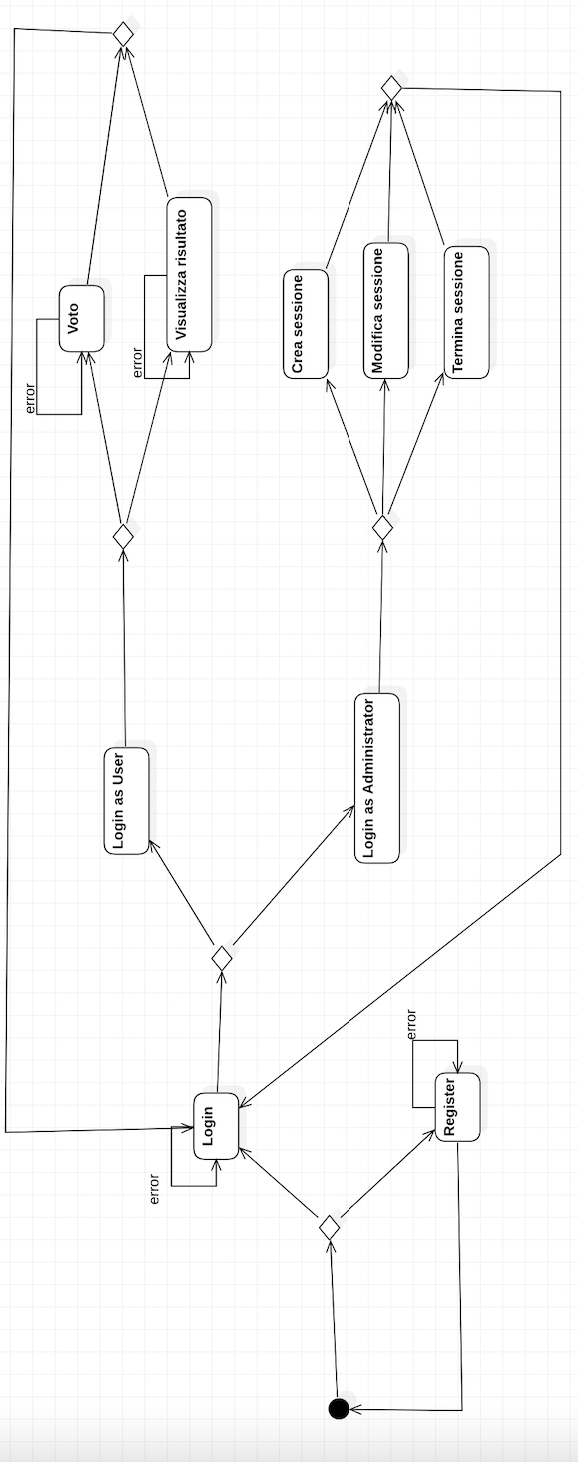
\includegraphics[scale=0.7]{images/uidiagram.png}\\
    \emph{easyVote's UI description diagram}
    \end{center}
    \pagebreak

\section{Specification and validation of JML}
The signatures of functions and methods of the easyVote project were complemented with specification and validation using the JML and Javadoc (using the \href{https://google.github.io/styleguide/javaguide.html}{google style} of Javadoc) a few snippets are:
\begin{itemize}
    \item In the context of dates during the registration process:\\
    \emph{Invariants:} self.giorno $>$ 0 and self.giorno $<$ 32, self.mese $>$ 0 and self.mese $<$ 13, self.anno $>$ 1800
    \item In the context of dates during in the session definition process:\\
    \emph{Invariants:} self.giorno $>$ 0 and self.giorno $<$ 32,  self.mese == 2 implies self.giorno $<$ 30, self.mese == 4 or self.mese == 6 or self.mese == 9 or self.mese == 1
    \item in the context of users:\\
    \emph{Pre-conditions:} username != null and password != null
\end{itemize}

\pagebreak

\section{User interface description}
\subsection{Landing page}
Form at the opening of the program
    \begin{center}
    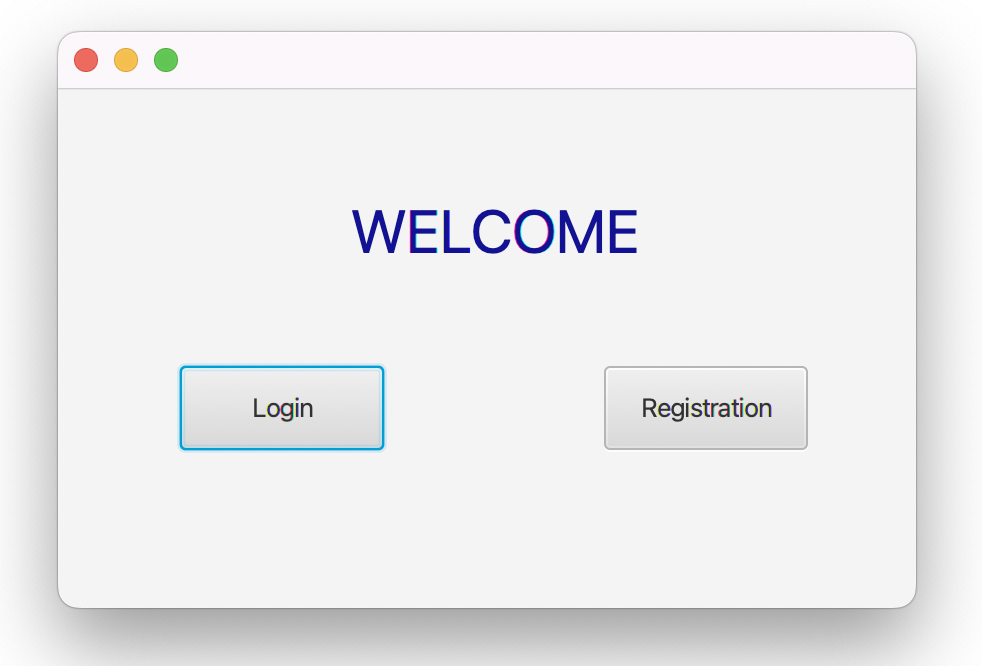
\includegraphics[scale=0.5]{images/ui1.png}\\
    \emph{Landing page}
    \end{center}
\subsection{Registration page}
Form to register a new user
    \begin{center}
    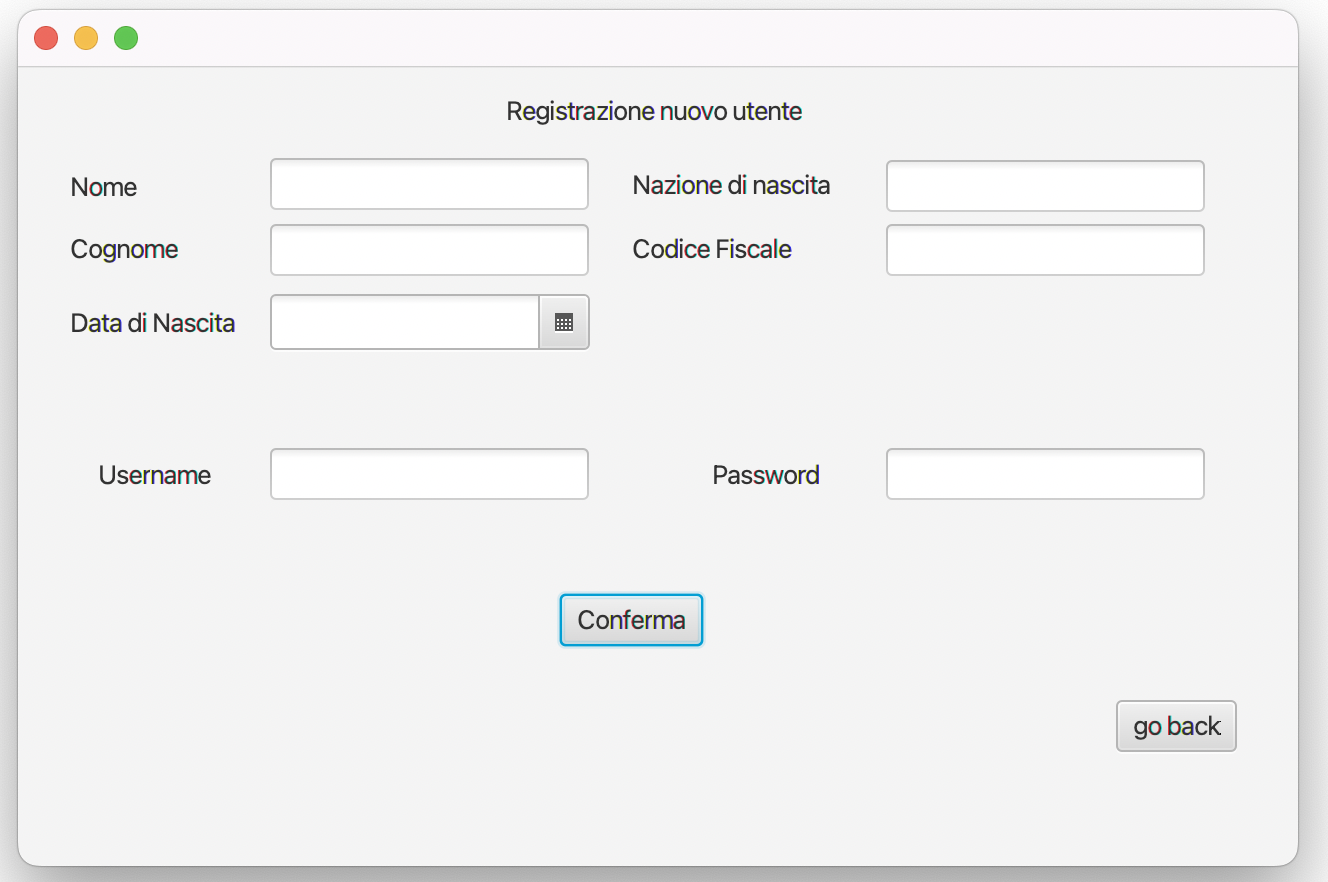
\includegraphics[scale=0.5]{images/ui2.png}\\
    \emph{Registration page}
    \end{center}
\subsection{Login page}
Form to login a user
    \begin{center}
    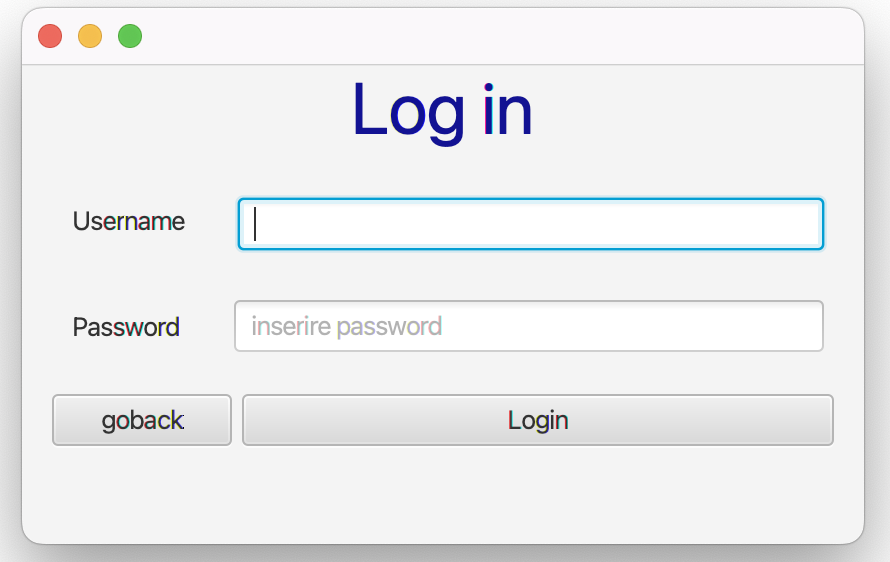
\includegraphics[scale=0.75]{images/ui3.png}\\
    \emph{Login page}
    \end{center}
\subsection{Activity page}
Form to select the activity that a user wants to make as an admin
    \begin{center}
    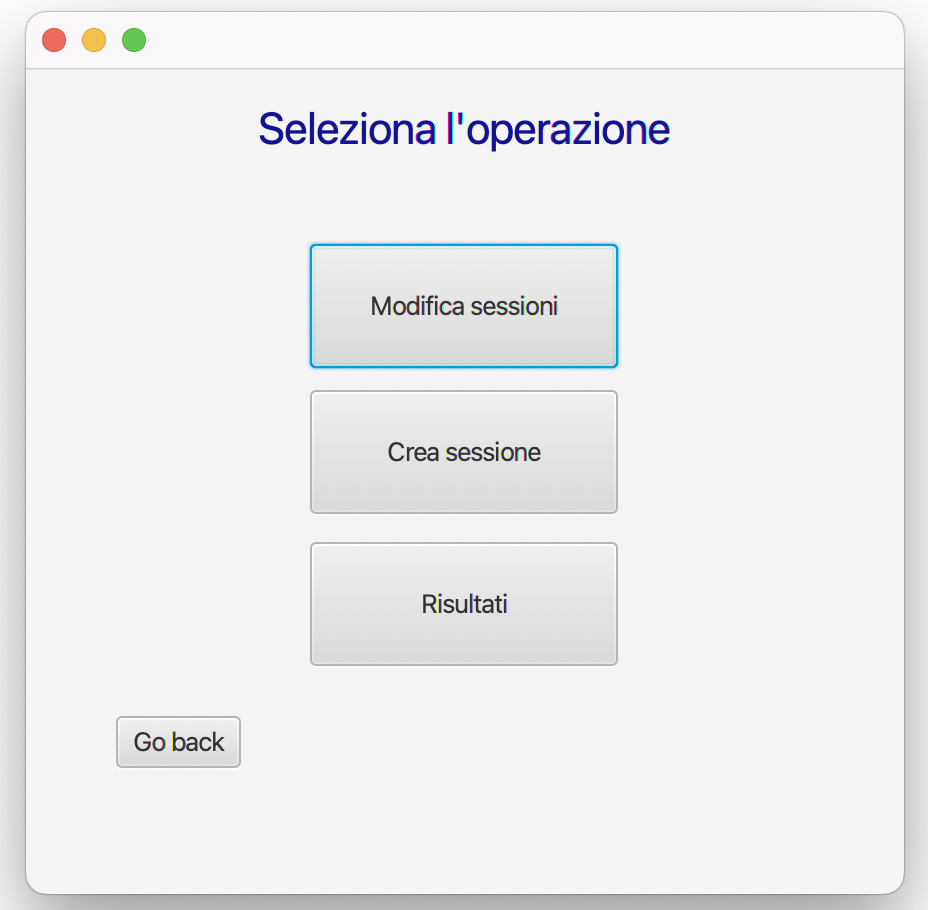
\includegraphics[scale=0.45]{images/ui4.png}\\
    \emph{Activity page}
    \end{center}
\subsection{Session modification page}
Form to select the session upon which an admin wants to make modifications
    \begin{center}
    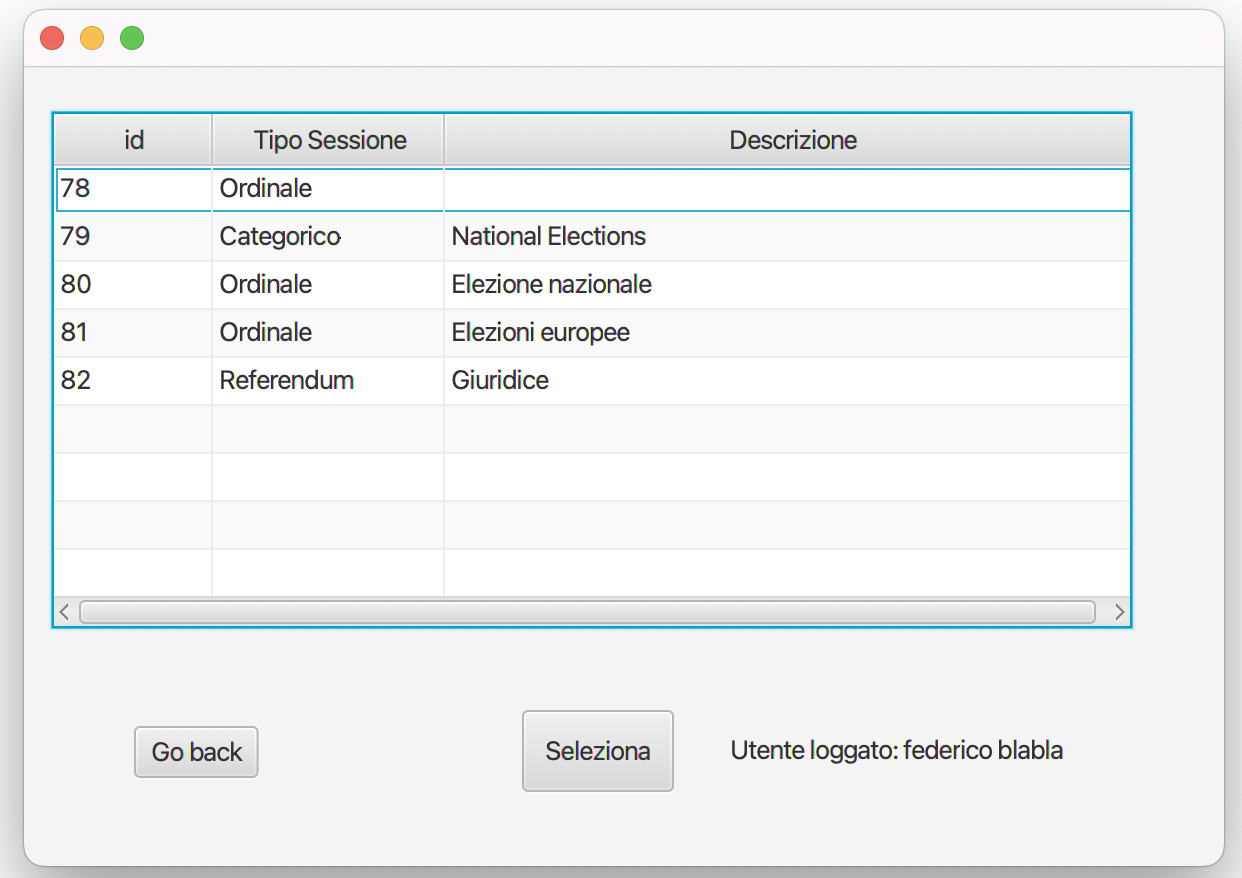
\includegraphics[scale=0.5]{images/ui5.png}\\
    \emph{Session modification page}
    \end{center}
\subsection{Session creation page}
Form to create a new voting session
    \begin{center}
    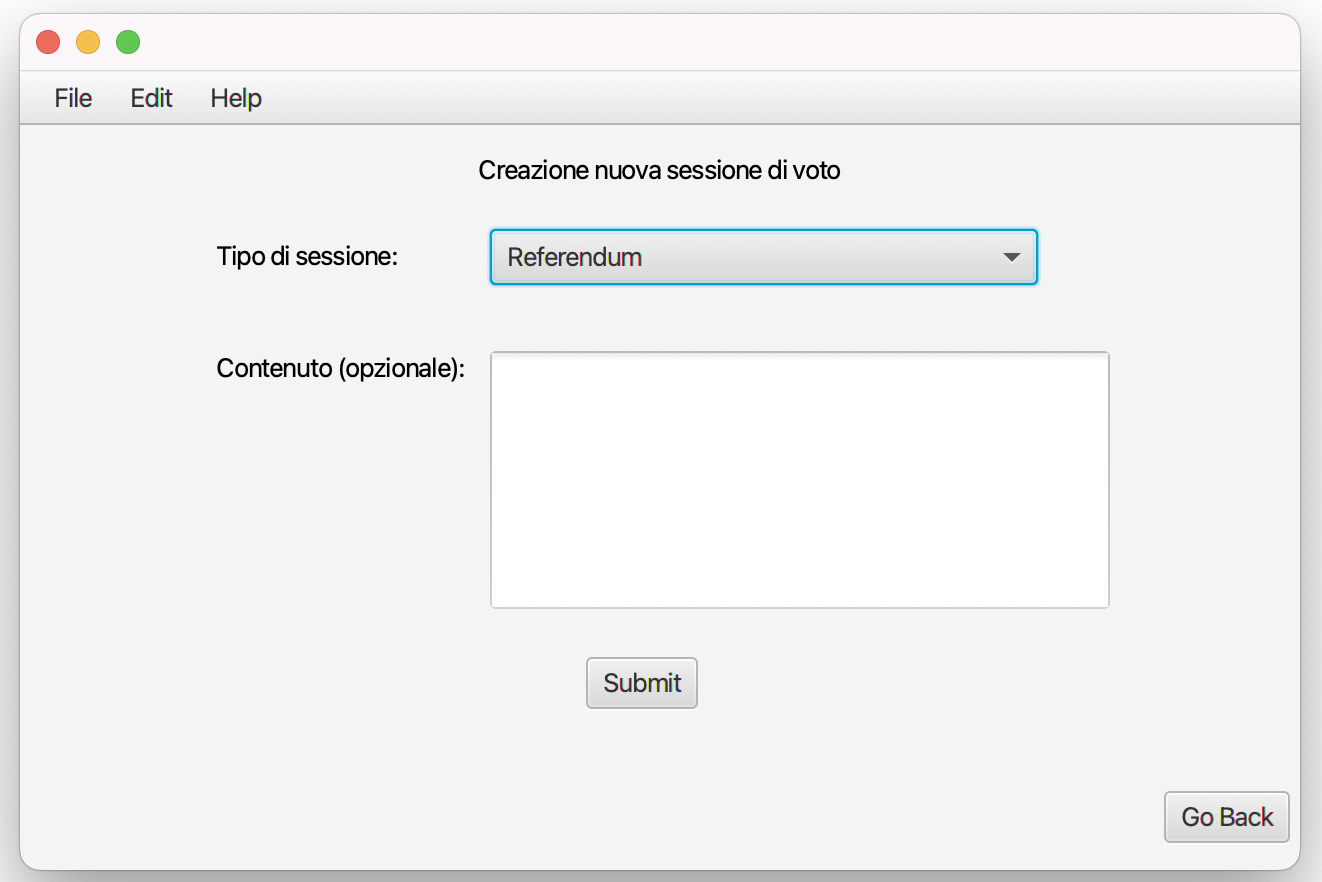
\includegraphics[scale=0.45]{images/ui6.png}\\
    \emph{Session creation page}
    \end{center}
\subsection{Session properties definition page}
Form to set the candidates, description and remove candidates from a created voting session
    \begin{center}
    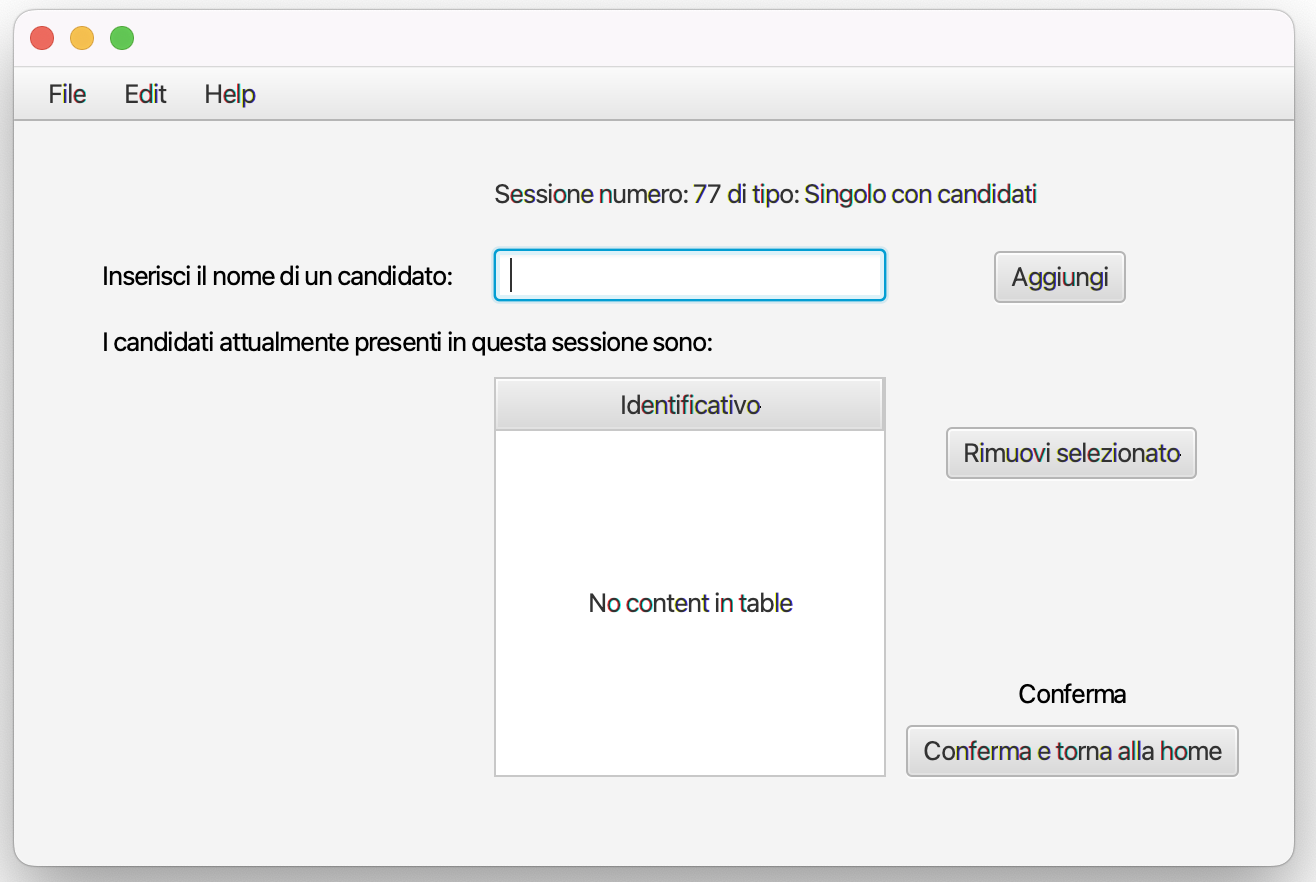
\includegraphics[scale=0.6]{images/ui7.png}\\
    \emph{Session properties definition page}
    \end{center}
    
\pagebreak
\subsection{Action selection page}
Form to select which operation a user wishes to make as logged user
    \begin{center}
    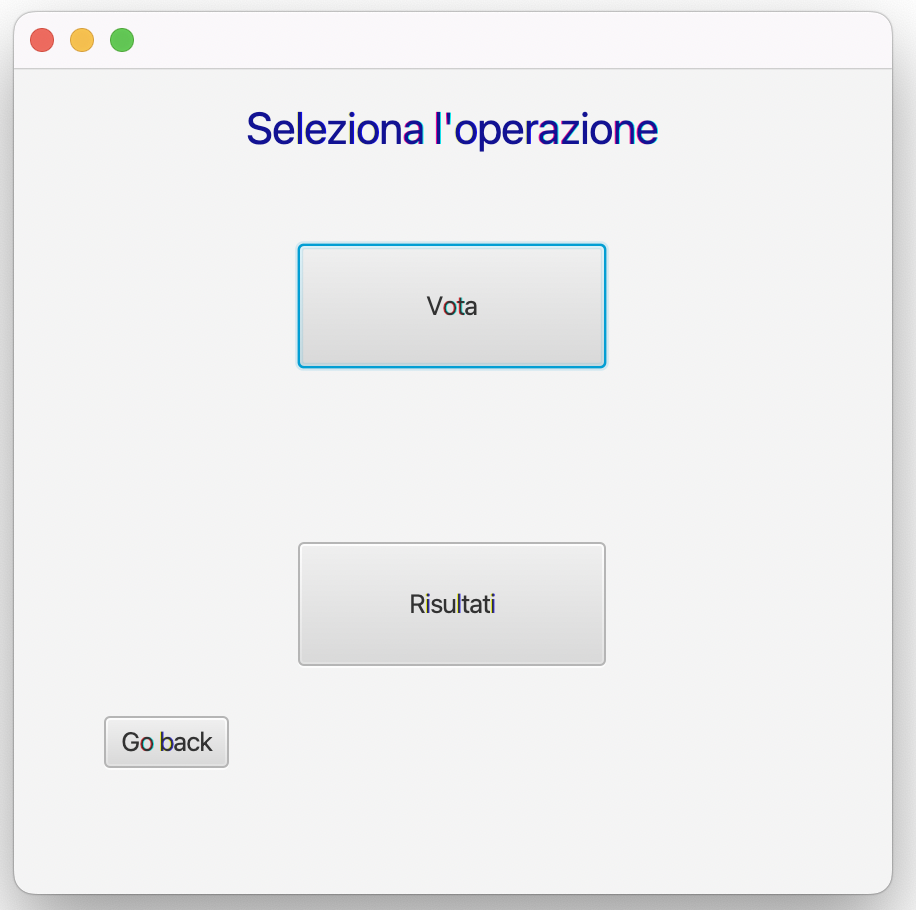
\includegraphics[scale=0.4]{images/ui8.png}\\
    \emph{Action selection page}
    \end{center}
\subsection{Session selection page}
Form to select the session in which the logged user wants to vote in
    \begin{center}
    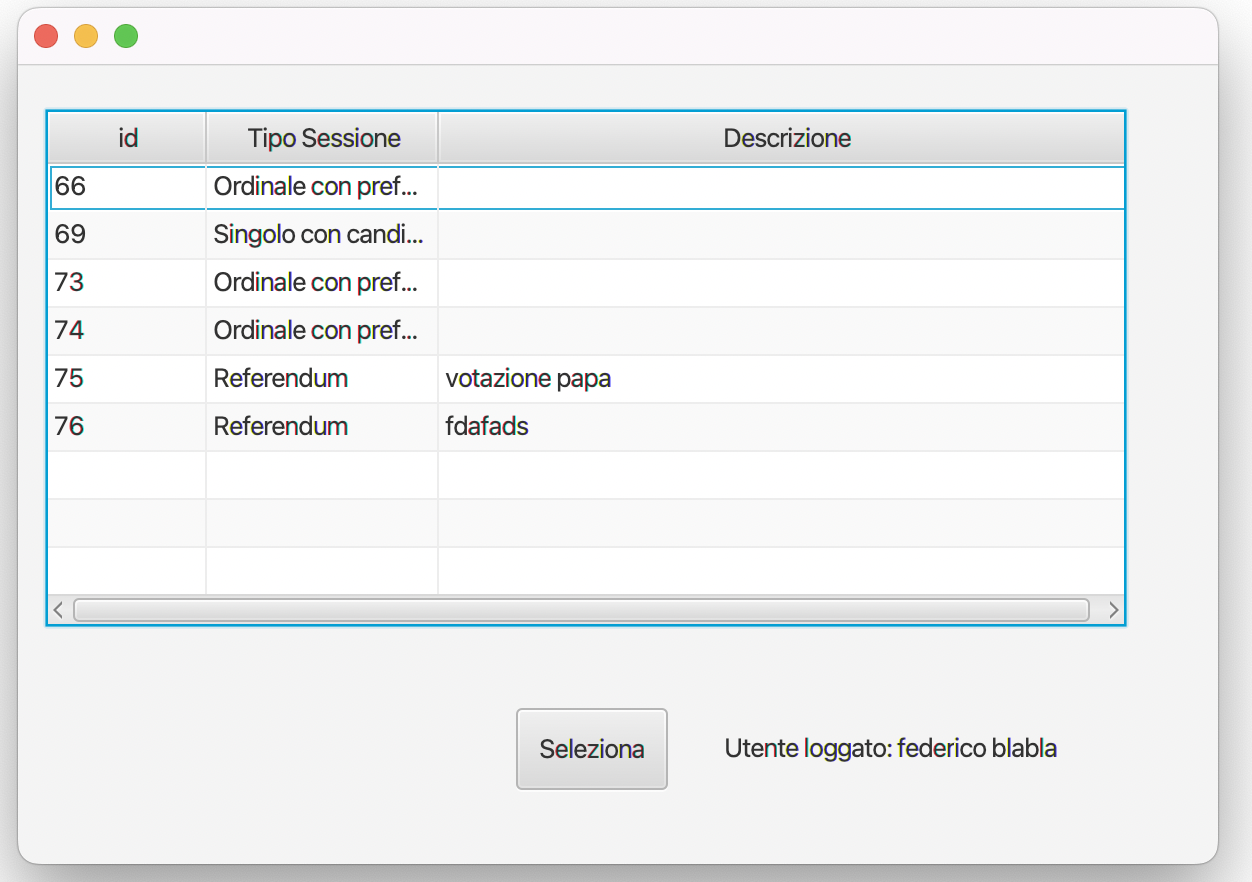
\includegraphics[scale=0.5]{images/ui9.png}\\
    \emph{Session selection page}
    \end{center}
\subsection{Preferential vote page}
Form to vote in a preferential voting session as a logged user
    \begin{center}
    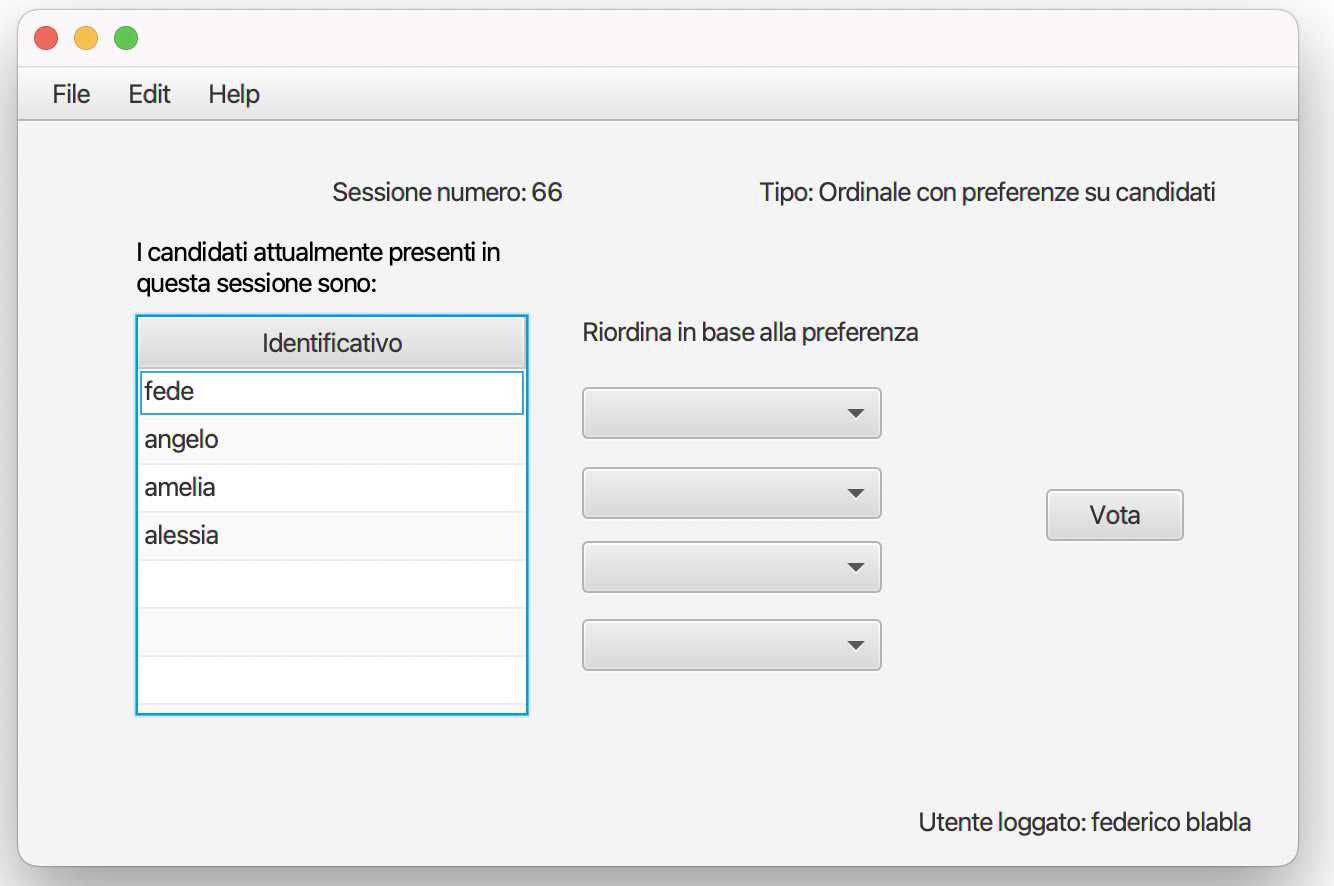
\includegraphics[scale=0.45]{images/ui10.png}\\
    \emph{Preferential vote page}
    \end{center}
\subsection{Referendum vote page}
Form to vote in a referendum voting session as a logged user
    \begin{center}
    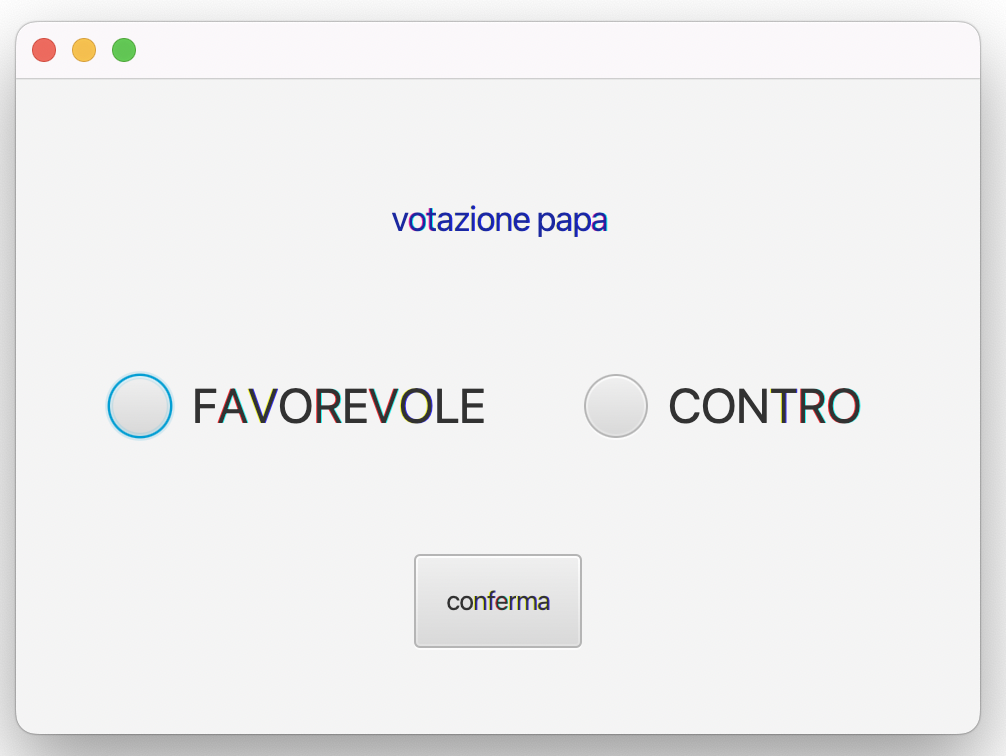
\includegraphics[scale=0.5]{images/ui11.png}\\
    \emph{Referendum vote page}
    \end{center}
\subsection{Categorical vote page}
Form to vote in an categorical voting session as a logged user
    \begin{center}
    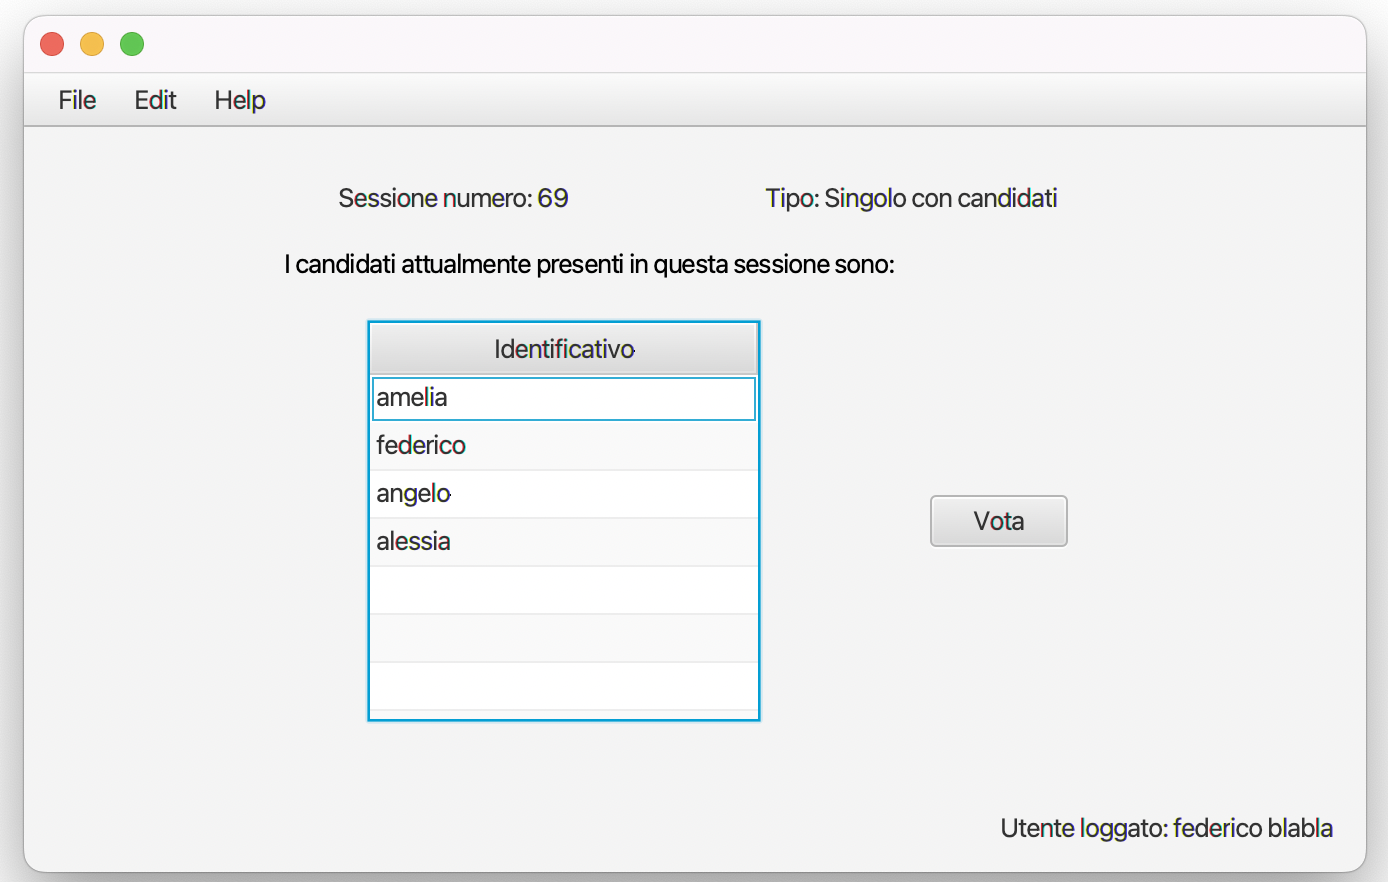
\includegraphics[scale=0.45]{images/ui12.png}\\
    \emph{Categorical vote page}
    \end{center}
\subsection{Categorical vote results page}
Form to display the results of an categorical voting session as an admin
\begin{center}
    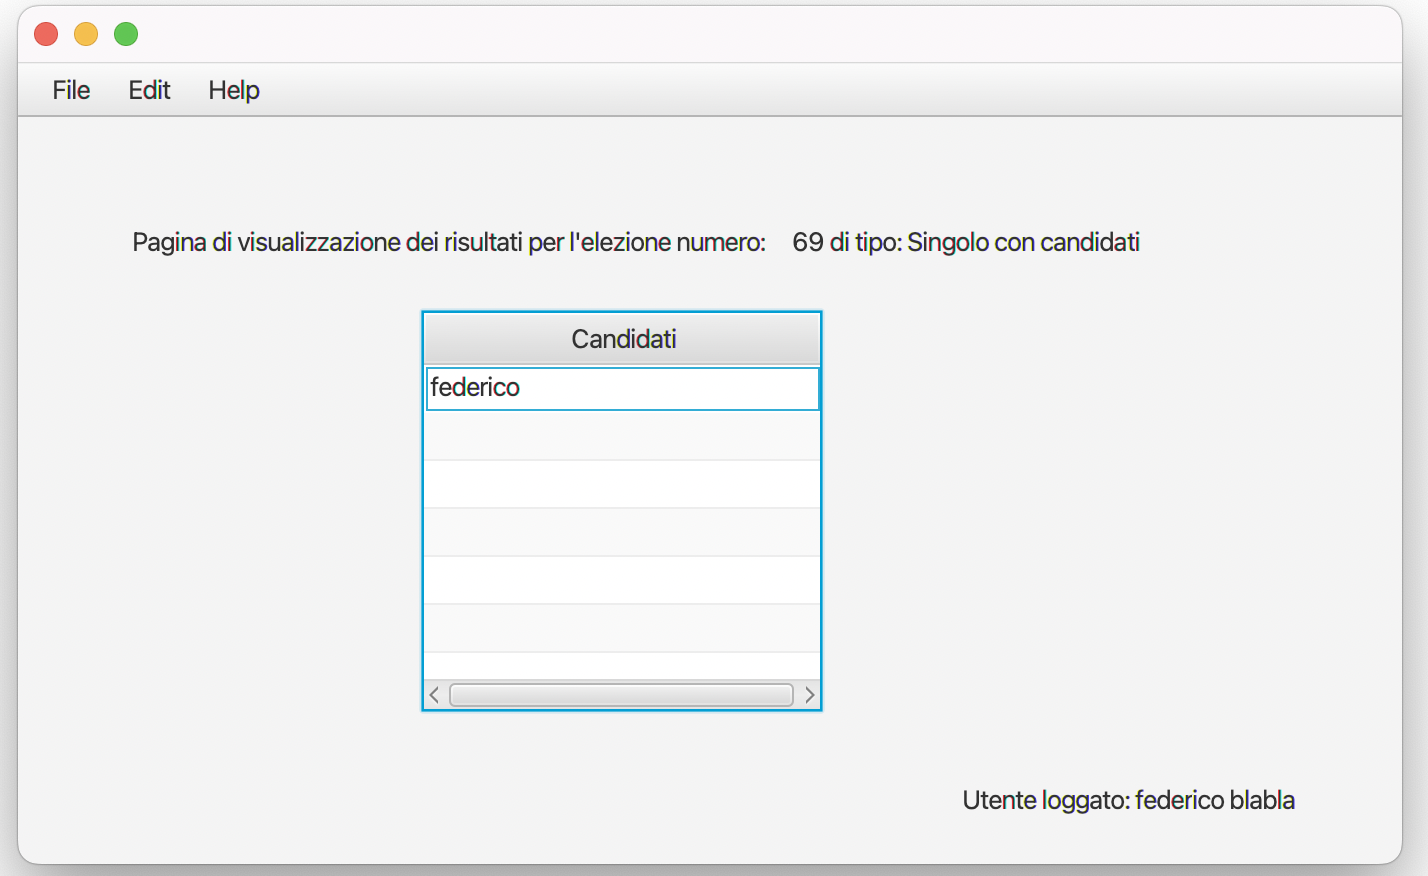
\includegraphics[scale=0.5]{images/ui13.png}\\
    \emph{Categorical vote results page}
    \end{center}
\subsection{Referendum vote results page}
Form to display the results of a referendum voting session as an admin
\begin{center}
    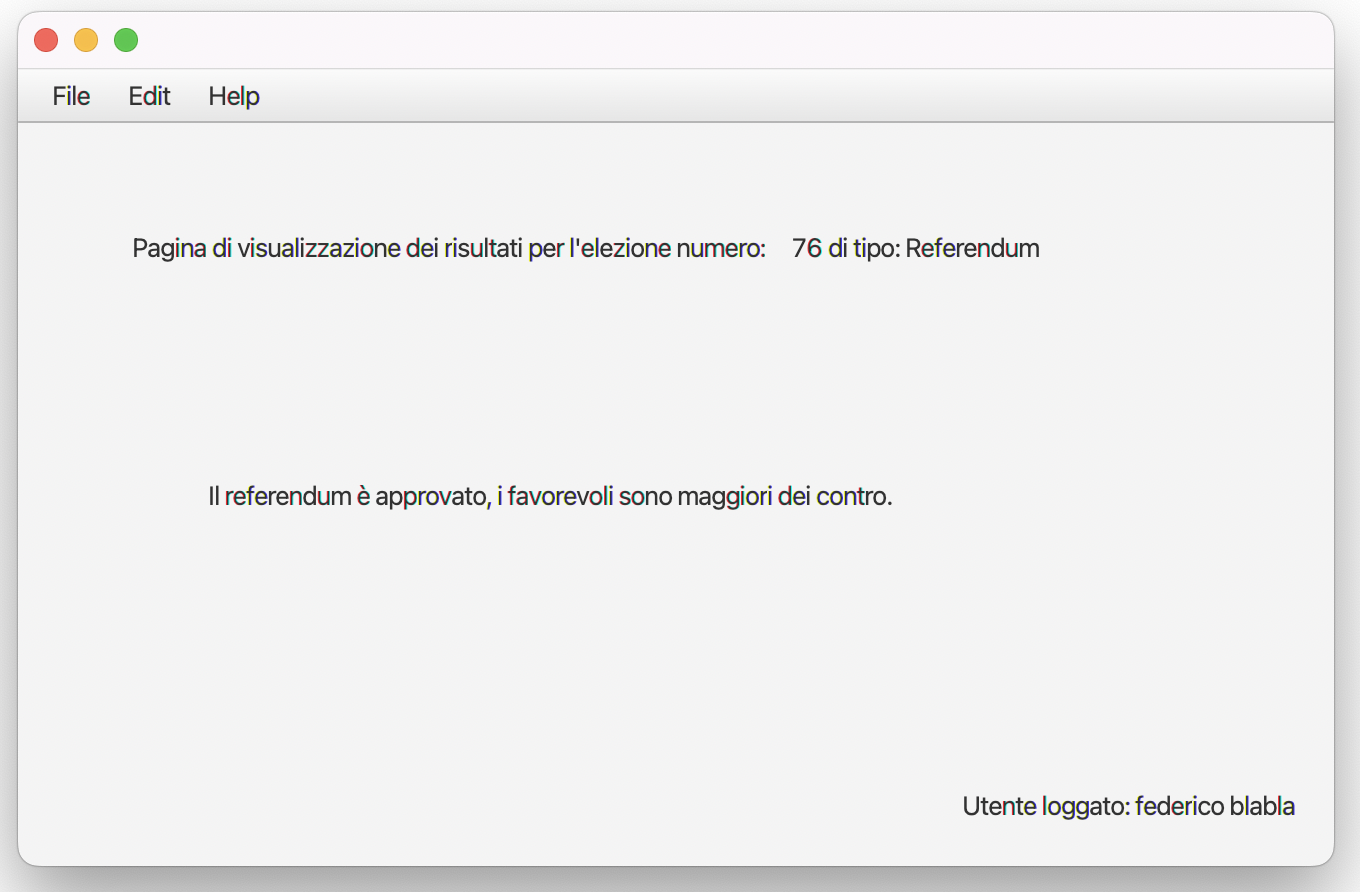
\includegraphics[scale=0.45]{images/ui14.png}\\
    \emph{Referendum vote results page}
    \end{center}

\pagebreak

\section{Testing}

The easyVote project was tested thoroughly and extensively with JUnit.
Testing was done on the following aspects:
\begin{itemize}
    \item User registration
    \item User login
    \item User deletion
    \item Admin registration
    \item Admin login
    \item Admin deletion
    \item Open session visualization
    \item Session creation
    \item Session modification
    \item Session deletion
    \item Voting in a referendum
    \item Voting in an ordinary session
    \item voting in a simple voting session
    \item Session results display
\end{itemize}
and many more.


\pagebreak


\section{Installation mode and settings}

The easyVote project can be found in the \href{https://github.com/junxiangfederico/easyVote}{Github repository}.
Please follow these tips:
\begin{itemize}
    \item Make sure you are using Eclipse as your IDE.
    \item Make sure to build using the following "VM Arguments": \emph{--module-path "yourPath" --add-modules
javafx.controls,javafx.fxml}, where "yourPath" refers to your path to the JavaFX folder.
    \item If the program is unable to start, try to call the command:
    \emph{mvn eclipse:eclipse}
    \item Import the "MySQL" database under "/easyVote/database". You can access administrator utilities using the username "bloblo" and password "bloblo".
\end{itemize}
\end{document}

